\documentclass{atlasnote} 


%\documentclass[usetikz]{atlasnote} % the 'usetikz' option loads tikz.sty in the proper place, 
                                   % avoiding conflicts with graphicx.sty.
                                   % Don't know what tikz.st is? Just ignore this line! :-)

%\documentclass[coverpage]{atlasnote} % the 'coverpage' option loads the ATLAS Cover Page package 
                                      % ans makes sure that the cover page is generated before the
                                      % note title page. Make sure that the latest version of
                                      % of 'atlascover.sty. is installed on your system!

%\usepackage{graphicx} % This is already loaded by the atlasnote class
                       % Just use it to include your plots!


\usepackage[section] {placeins}% to prevent "too many unprocessed floats" error. Lily.


% default location 
\graphicspath{{./figures/}}

\usepackage{amsmath}
\usepackage{atlasphysics}
\usepackage{url}
%\usepackage{subfigure}
\usepackage{caption}
\usepackage{subcaption}
\usepackage{epstopdf}
\usepackage{multirow}
\usepackage{xspace}
\usepackage{atlasphysics}
\usepackage{rotating} 
\usepackage{longtable}
\usepackage{multirow}
\usepackage{url}
\usepackage{setspace}

\usepackage{hyperref}
\hypersetup{
  colorlinks=true,
  linkcolor=blue,
  citecolor=blue,
  urlcolor=blue
}

% define some useful shortcuts
\newcommand\fb{$\mathrm{fb}^{-1}$}
\newcommand\Zgamma{$Z\gamma$}
\newcommand\HToZg{$H \to Z\gamma$\ }
\newcommand\dm{\ensuremath{\Delta m}\ }
\newcommand\ZBoson{$Z$\ }
\newcommand\WBoson{$W$\ }
\newcommand\WBosons{$W^{\pm}$\ }
\def\LL    {\ensuremath{\mathcal{L}}}
\def\vecth {\ensuremath{\boldmath \theta}}
\newcommand\mll {\ensuremath{m_{\ell \ell}}\ }
\newcommand\mllg{\ensuremath{m_{\ell \ell \gamma}}\ }
\newcommand{\mbf}{\mathbf}
\newcommand{\tabscript}[3]{%
 	\setlength{\fboxrule}{0pt}%
 	\fbox{\ensuremath{#1^{#2}_{#3}}}%
}%for super and sub scripts  in tabulars
\def\progname#1{{\sc #1}}
\def\brocket#1{\left\langle #1 \right\rangle}
\newcommand{\refF}[1]{Figure \ref{#1}}
\newcommand{\refT}[1]{Table \ref{#1}}
\newcommand{\refS}[1]{Section \ref{#1}}
\newcommand{\refC}[1]{Chapter \ref{#1}}
\newcommand{\refA}[1]{Appendix \ref{#1}}
\newcommand{\refE}[1]{(\ref{#1})}
%% \renewcommand{\labelitemi}{-}

%%%%%%% Analysis numbers %%%%%%%
\newcommand\lumiseventev{4.6}
\newcommand\lumieighttev{20.7}
\newcommand\totlumieighttev{20.7}
\newcommand\lumierrseventev{0.1}
\newcommand\lumierreighttev{0.7}

\newcommand\pval{\ensuremath{p_0}}

% min observed p-value
\newcommand\pvaluelow{0.042}
% max observed p-value
\newcommand\pvaluehigh{0.966}
% observed p-value at 125 GeV
\newcommand\pvaluehiggs{0.188}
% observed p-value at 126.5 GeV
% \newcommand\pvaluehiggs{0.468}
% min observed significance
\newcommand\sigmalow{-1.83}
% max observed significance
\newcommand\sigmahigh{1.61}
% observed significance at 125 GeV
\newcommand\sigmahiggs{0.89}
% observed significance at 126.5 GeV
% \newcommand\sigmahiggs{0.08}
% min expected p-value
\newcommand\pvaluelowexp{0.40}
% max expected p-value
\newcommand\pvaluehighexp{0.46}
% expected p-value at 125 GeV
\newcommand\pvaluehiggsexp{0.443}
% expected p-value at 126.5 GeV
%\newcommand\pvaluehiggsexp{0.440}
% min expected significance
\newcommand\sigmalowexp{0.25}
% max expected significance
\newcommand\sigmahighexp{0.26}
% expected significance at 125 GeV
\newcommand\sigmahiggsexp{0.14}
% expected significance at 126.5 GeV
% \newcommand\sigmahiggsexp{0.15}
% min expected exclusion
\newcommand\excllowexp{7.3}
% max expected exclusion
\newcommand\exclhighexp{22}
% expected exclusion at 125 GeV
\newcommand\exclhiggsexp{13.5}
% expected exclusion at 126.5 GeV
% \newcommand\exclhiggsexp{12.5}
% min observed exclusion
\newcommand\excllow{5.4}
% max observed exclusion
\newcommand\exclhigh{37}
% observed exclusion at 125 GeV
\newcommand\exclhiggs{18.2} 
% observed exclusion at 126.5 GeV
%\newcommand\exclhiggs{12.9}
% exclusion without syst errors, at 125 GeV
\newcommand\exclhiggsnosyst{17.4}
\newcommand\exclhiggsexpnosyst{12.9}

%%%%%%%%%%%%%%%%%%%%%%%%%%%%%%%%%%%%
%           Title page             % 
%%%%%%%%%%%%%%%%%%%%%%%%%%%%%%%%%%%%

%\skipbeforetitle{10pt}

%\atlasnote{1.0} 

\title{\boldmath Search for the Standard Model Higgs boson in the $H \ra Z\gamma$ decay mode with $pp$ collisions at $\sqrt{s}=7$ and $8$ TeV}

\usepackage{authblk}
\renewcommand\Authands{, } % avoid ``. and'' for last author
\renewcommand\Affilfont{\itshape\small} % affiliation formatting

\author[a]{Joshua Loyal}

\affil[a]{Duke University, Physics Department}



% Date: if not given, uses current date
\date{\today}

% Draft version: if given, adds draft version on front page, a
% 'DRAFT' box on top of each other page, and line numbers to easy
% commenting. Comment or remove in final version.
\draftversion{1.0}

% Journal: adds a 
%\journal{Phys. Lett. B} 

\doublespacing

% Abstract
\abstracttext{
\singlespacing
The ATLAS and CMS collaborations have observed a Higgs-like boson
with a measured mass of 125.2 $\pm$ 0.3 (\emph{stat}) $\pm$ 0.6 (\emph{sys}) GeV 
using data taken from the Large
Hadron Collider (LHC) in Geneva, Switzerland. Now it is important to understand
the various properties of the Higgs-like resonance using all of the available
information provided by the ATLAS experiment. As such, a search for the Standard
Model Higgs boson in the decay channel \HToZg, $Z\ra\ell^+\ell^-$, where
$\ell = e$ or $\mu$, was conducted using proton-proton collisions recorded
with the ATLAS detector at the LHC. The distribution of the difference \dm between 
the final state three-body mass \mllg and the di-lepton invariant mass \mll
is compared to Standard Model (SM) background expectations. No significant
deviation from the SM prediciton is observed and upper limits on the 
cross-section of a Standard Model Higgs boson with a mass between 120 and 150 GeV
are derived. The expected exclusion limits at 95\% confidence level range between
\excllowexp\ and \exclhighexp\ times the predicted Standard Model
cross section.
The observed exclusion limits range between \excllow\ and \exclhigh\
times the Standard Model cross section.
For a Higgs boson mass of 125 GeV, the expected and observed limits
are \exclhiggsexp\ and \exclhiggs\ times the Standard Model, respectively.
}

%%%%%%%%%%%%%%%%%%%%%%%%%%%%%%%%%%%%
%            Content               % 
%%%%%%%%%%%%%%%%%%%%%%%%%%%%%%%%%%%%

\begin{document}

%% Some variable definitions

%%%%%%%%%%%%%%%%%%%%%%%%%%%%%%%%%%%%%%%%%%%%%%%%%%%
% isEM variables
%
% Hadronic leackage
\newcommand{\Rhad}    {\ensuremath{R_{\rm had}}}
\newcommand{\Rhadone} {\ensuremath{R_{\rm had_{1}}}}

% Middle
\newcommand{\Reta}    {\ensuremath{R_{\eta}}}
\newcommand{\Rphi}    {\ensuremath{R_{\phi}}}
\newcommand{\wetatwo} {\ensuremath{w_{2}}}

% Strips
\newcommand{\Fside}   {\ensuremath{F_{\rm side}}}
\newcommand{\wthree}  {\ensuremath{w_{s\,3}}}
\newcommand{\wtot}    {\ensuremath{w_{s\,{\rm tot}}}}
\newcommand{\DeltaE}  {\ensuremath{\Delta{}E}}
\newcommand{\Eratio}  {\ensuremath{E_{\rm ratio}}}
\newcommand{\Emaxtwor}{\ensuremath{R_{\rm max\,1}}}
%%%%%%%%%%%%%%%%%%%%%%%%%%%%%%%%%%%%%%%%%%%%%%%%%%%

\newcommand{\mo}      {\ensuremath{^{-1}}}

\newcommand{\Etg}     {\ensuremath{E_{T}^{\gamma}}}

%%%%%%%%%%%%%%%%%%%%%%%%%%%%%%%%%%%%%%%%%%%%%%%%%%%
%for efficiency section
\newcommand{\effID}{\hbox{$\varepsilon^{{\rm offl}}$}}
\newcommand{\effReco}{\hbox{$\varepsilon^{{\rm reco}}$}}

%%%%%%%%%%%%%%%%%%%%%%%%%%%%%%%%%%%%%%%%%%%%%%%%%%%
%for purity section
\newcommand{\EtCone}{\et^{(R<0.4)}}

\newcommand{\obs}{^\mathrm{obs}}
\newcommand{\sig}{^\mathrm{sig}}
\newcommand{\bkg}{^\mathrm{bkg}}
\newcommand{\Ns}{N\sig}
\newcommand{\Nb}{N\bkg}
\newcommand{\N}{N\obs}

\newcommand{\pdf}{\Pi}
\newcommand{\ph}{_\gamma}
\newcommand{\MC}{_\mathrm{MC}}
\newcommand{\data}{_\mathrm{data}}

\newcommand{\etaM}{|\eta_\mathrm{S2}|}

\newcommand{\ptjet}{p_{T}(\mathrm{jet})}
\newcommand{\ntrk}{N(\mathrm{tracks})}

\newcommand{\Equation}[2]{\begin{equation} #2 \label{#1} \end{equation} }
%%%%%%%%%%%%%%%%%%%%%%%%%%%%%%%%%%%%%%%%%%%%%%%%%%%


\tableofcontents

\newpage

% - Theoretical introduction and motivation
% - Idea behind the ATLAS experiment and search
% - Future use of this information

\section{Introduction} % (non-mathematical)
% Breif introduction to the Standard Model and Gauge Symmetries 

% Motivation for spontaneous symmetry breaking / the higgs mechanism

% The current status of the Higgs search

% Motivation for searching for H->Zg

% The ATLAS experiment and the form of the measurement, 
% i.e. how and what is measured

Elementary particle physics addresses the question, `What is the world made of?' 
at the most fundamental level, i.e. on the smallest scale of size. 
One could easily imagine a world where the elementary building blocks of 
nature come in a vast variety of shapes and sizes. Just think of the multitude of 
parts that work together to make up an ordinary car. Remarkably this is not
the case. The tiniest chunks of nature come in a small number of different types
(electrons, quarks, photons, and so on), which are replicated in astronomical
quantities to form our macroscopic world. This is not the whole story.
Not only is elementary particle physics concerned with identifying the various 
fundamental actors of nature, but also how these actors interact amongst each other.
It is during this investigation that the familiar forces of nature make their
appearance. This paper is concerned with measuring both of these phenomena through 
a search for a new particle known as the Higgs boson as well as an investigation of
how this particle interacts with two other important actors: the photon and the 
$Z$ boson.

On July 4th, 2012 the ATLAS and CMS collaborations both announced the 
discovery of a particle consistent with the 
Standard Model Higgs boson~\cite{ATLAS_Higgs,CMS_Higgs}, indicating that
the discovery of the mechanism behind spontaneous symmetry breaking in the
Standard Model may be at hand. In addition, the ATLAS experiment measured 
this Higgs-like boson's mass to be close to 125 GeV~\cite{ATLAS_Higgs_Dec12}.
This measurement is only the beginning of a challenging program of `Higgs
identification' through which the consistency of this new boson with the SM
Higgs will be verified or disproved. For this reason it is now becoming
increasingly important to measure the properties of this new scalar particle
as well as its rate of decay for the largest number of experimentally
viable decay channels. These analyses could result in tension with the SM
Higgs prediction, for instance the rate of one or more measured decay channels
may differ from the SM prediction. The simplest mechanism for such a scenario
is an enhancement/suppression in loop-induced decays
\footnote{A loop means that particles of any mass can instantly materialize and 
then disappear during the decay process. The brief-lived virtual particles
are usually $W$ bosons, but other particles with similar behavior can enter
the loop, including many beyond the Standard Model particles. This makes decays 
involving loops very sensitive to new physics at high masses.}
that are naturally sensitive to couplings to new virtual particles, 
for instance the decay \HToZg presented in this paper. 
This would thus be evidence for Beyond the Standard Model (BSM) physics.

The main decay modes being probed in the searches
presented during the July 4th announcement are the $H \to \gamma\gamma$ channel,
the $H \to WW^* \to 2\ell2\nu$ channel and the 'golden channel',
$H \to ZZ^* \to 4\ell$. However, little attention has been paid to the 
$H \to Z\gamma \to \ell^+\ell^-\gamma$ channel
despite the fact that its event rate is comparable to that of the golden channel 
for a 125 GeV Standard Model Higgs boson. The main reason for this is 
the low branching ratio for $Z \to \ell^+\ell^-$, the
probability that a $Z$ boson will decay into two leptons, 
makes the $Z\gamma$ channel statistically limited. 
Although, the background rate, the number of non-interesting physics processes
that contaminate the process of interest, of the $Z\gamma$ channel is higher than
that of the $ZZ^* \rightarrow 4\ell$ channel
there are a few important properties that make a study of the $Z\gamma$ channel 
compelling: 
1) all final state particles can be measured well with the ATLAS detector;  
2) the Higgs mass could be measured from the total invariant mass spectrum; 
3) the spin of the Higgs can be studied by analyzing the angular distribution 
of the decay products, and 
4) this channel can be used for setting limits on the Higgs coupling constants.
In addition, the ratio of $\gamma\gamma$ to $Z\gamma$ branching ratios can
be used to discriminate between certain models of 
new physics~\cite{Zg_newPhy_1,Zg_newPhy_2, Zg_newPhy_3}.
All of these measurements will help to identify this new particle sitting
close to 125 GeV as a Standard Model Higgs boson or something more exotic.

% re-write this with my own words....
This report documents the measurements of the \HToZg production rate observed
using data from $pp$ collisions provided by the LHC. In the following, the
theory behind the \HToZg decay is discussed in Section~\ref{sec:theory},
the ATLAS detector is described in Section~\ref{sec:atlas}, and the signal
and backgrond simulation samples used in the analysis are presented in
Section~\ref{sec:sigbkg}. The event selection criteria are described in 
Section~\ref{sec:event}. A comparison between the selected data sample and
the simulation is presented in Section~\ref{sec:compare}. The discrimination
between signal and background events is performed by means of an unbinned
maximum likelihood fit, and the estimated signal yield is compared to the one 
predicted by the Standard Model. The properties of the signal, in terms of
the expected yields and the signal model used for the fit are described
in Section~\ref{sec:signal}, while the choice of the background model adopted
in the fit is motivated in Section~\ref{sec:background}. After a description of
the systematic uncertainties in Section~\ref{sec:sys}, Section~\ref{sec:results}
presents the results of the combined analysis of the 7 and 8 TeV datasets.

\label{sec:intro}

\section{Theory}
\label{sec:theory}

This section is devoted to laying out a more formal description of the
theory presented in Section~\ref{sec:intro}. While the particles and
their properties tabulated in Figure~\ref{fig:sm} summarize the important
players in the study of elementary particles, an understanding of the
mathematical ideas behind the Standard Model's construction are essential in grasping
the importance of this measurement. This paper is focused on the measurement
of \HToZg at the LHC; therefore, a rigorous development of this ideas is forgone. 
For this see Halzen and Martin~\cite{QuarksLeptons}.

% Section~\ref{subsec:qed} gives a brief
% introduction to Gauge Theory and Quantum Field Theory through the simplest
% theory contained in the Standard Model: Quantum Electrodynamics (QED).
% Afterward the Higgs Mechanism is explained in Section~\ref{subsec:higgsmec}
% and finally the production processes studied in this measurement are
% given in Section~\ref{subsec:prodproc}.


\subsection{The Role of Symmetry in Particle Physics}
\label{subsec:symmetry}

An important principle motivating the mathematical structure of modern physical 
theories is the notion of symmetry. On a macroscopic scale one can study
the interactions of objects by holding them at various
distances apart and measuring the force between them. That is how Coulomb derived
the famous inverse square law describing electric repulsion and attraction that
now bears his name. On the smallest scales this empirical data is no longer
available, so that a new paradigm is need to understand how these interactions
come about. 

A beautiful solution was brought to light by the brilliant 
mathematician and physicist Emmy Noether who showed that every symmetry in
nature leads to a conserved quantity, a value that does not change over time.
A familiar application of this connection is found in Newton's third law:
For every action there is an equal and opposite reaction. From this balancing of
forces one can derive a conserved quantity associated with the system's 
motion, namely momentum. The importance of Noether's approach using symmetries
is that it allows the physicist to turn this reasoning around. One can postulate
the existence of a symmetry of nature, in this case the invariance of the laws
of physics under translations in space, which leads to a conserved quantity (momentum)
that results in experimentally testable predictions (Newton's third law).

While quantities such as momentum are familiar at the macroscopic level, 
it turns out that similar symmetries exist at subatomic distances
known as internal symmetries. One of the first examples of these symmetries
known as isospin was put forth by Werner Heisenberg in 1932 
to explain the approximate symmetry between
the newly discovered neutron with its partner in the atomic nucleus, the proton.
This symmetry says that according to the strong interaction that holds
the nucleus together the neutron and proton are reflections of each other,
i.e. the exchange proton $\leftrightarrow$ neutron does not affect the
physics of the strong force. More importantly this symmetry predicts that the
scattering rates of the interactions
\begin{align*}
    & p + p \rightarrow \pi^+ + d \\
    & p + n \rightarrow \underbrace{\pi^0}_{\text{pion}} + \underbrace{d}_{\text{deuteron}}
\end{align*}
should be equal. The experimental verification of this prediction convinced
physicists that these internal symmetries can be used to study and predict
how particles interact at the smallest length scales.

Physicists now use similar internal symmetries known as gauge symmetries to
describe the fundamental particles and their interactions. These gauge symmetries
are mathematical constructs similar to isospin that predict force carrying 
particles that mediate interactions in a way that can be used to calculate
various measurable quantities. The current gauge-theory formulation which describes
much of the phenomena found in nature is known as the Standard Model.

\subsection{The Standard Model}
\label{subsec:StandardModel}
An picture of the Standard Model of particle physics is best obtained
by moving away from the abstract gauge-theory formulation and instead considering
the predictive outcomes of the theory. The Standard Model provides physicists with
the current answer to the question of what the world is made of and is displayed
in Figure~\ref{fig:sm}. This table is reminiscent
of the periodic table developed by chemists to explain the various atoms
found in nature. A surprising property of the Standard Model is that it consists
of only 16 different particles. There are six quarks, shown in purple, which
are the building blocks of the familiar nucleons, i.e. the proton and neutron.
Another six particles known as leptons, marked in green, include one of
the most familiar fundamental particles, the electron, 
which is responsible for the operation of most household circuits. And
finally there are the four gauge bosons highlighted in red, which are of the 
greatest relevance to the measurement presented in this paper.
The gauge bosons are responsible for mediating three 
out of the four fundamental forces in nature: the electromagnetic, strong, and 
weak interactions. As of now, theorists have been unable to incorporate the 
gravitational force, a pervasive component of the macroscopic world,
into the current gauge-theory of particle physics.

\begin{figure}[htbp]
    \centering
    \includegraphics[scale=0.4, angle=0]{./figures/StandardModelPNG}
    \caption{A table summarizing the particles described by the
    Standard Model of particle physics. The Standard Model encompasses
    three generations of quarks and leptons as well as four force carrying
    bosons.}
    \label{fig:sm}
\end{figure}

\subsection{The Higgs Mechanism}
\label{subsec:higgsmec}
The Higgs boson is an essential component of the Standard Model and plays
an important role in the predictive power of the theory. Like much of modern
physics, the Standard Model relies heavily on the symmetries of nature. Just
as concepts such as conservation of momentum and energy can be tied to the 
fact that a system is symmetric under translations in space and time\footnote{
This result is known as Noether's Theorem and can be attributed to the 
brilliant German mathematician Emmy Noether.}, much of the mathematical 
framework of the Standard Model is based on internal symmetries 
known as gauge symmetries. In fact there are three gauge symmetries found
in the Standard Model\footnote{ In group theoretic language the symmetries of
the Standard Model can be written as $SU(3) \times SU(2) \times U(1)$.} 
each of which predicts a force carrying particle that mediates one of the 
aforementioned interactions of nature. The photon mediates the 
electromagnetic interaction. The massless gluon is responsible for the strong 
interaction, which binds quarks together to form protons and neutrons.
And finally, the weak interaction, which causes radioactive decays, 
is mediated by the massive \WBosons and \ZBoson bosons. The problem with all 
of this symmetry is that it predicts that the weak nuclear force is a long
range force, something which is not observed in nature. The reason for this
discrepancy can be traced back to the fact that the \WBoson and \ZBoson bosons are
not massless particles, but have a mass of roughly 80 and 90 GeV respectively. 
In addition, these internal gauge symmetries also predict that other 
fundamental particles, such as the electron, are massless. In order to solve
this apparent predicament one needs to introduce a mechanism that keeps the
equations that govern the Standard Model's behavior symmetric, but allows for
some asymmetric lowest energy states, i.e. 'ground states'. 
This is accomplished with a theoretical mechanism known as spontaneous
symmetry breaking or in this special case the Higgs mechanism.

\subsection{Production Process}
\label{subsec:prodproc}

\begin{figure}[!htbp]
  \begin{center}
  {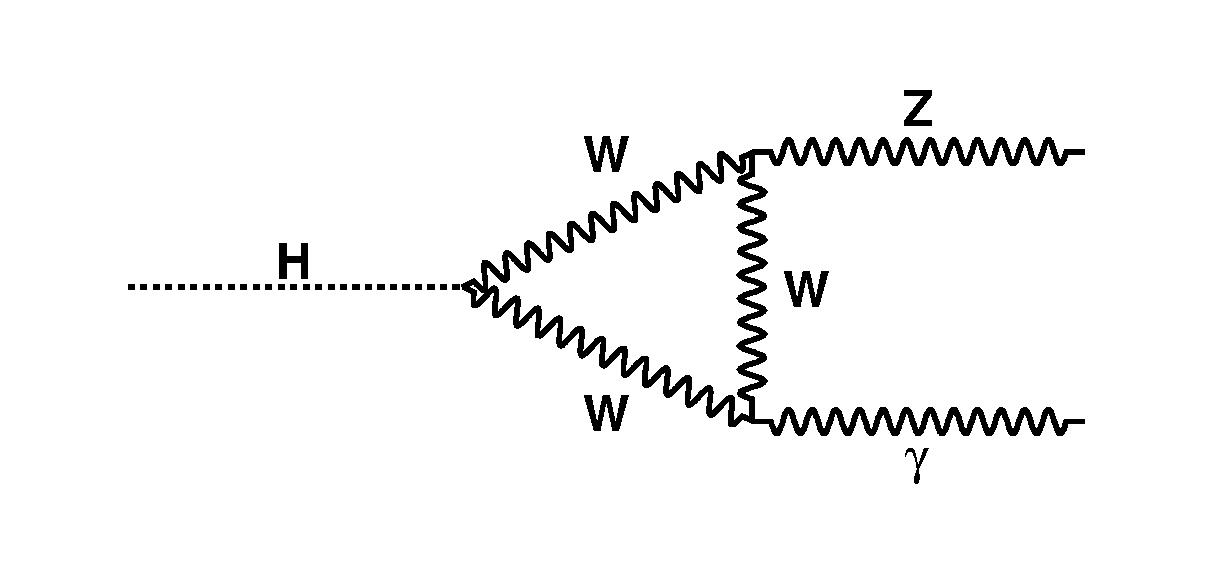
\includegraphics[width=2in]{figures/loop1}}
  {\includegraphics[width=2in]{figures/loop2}}
  {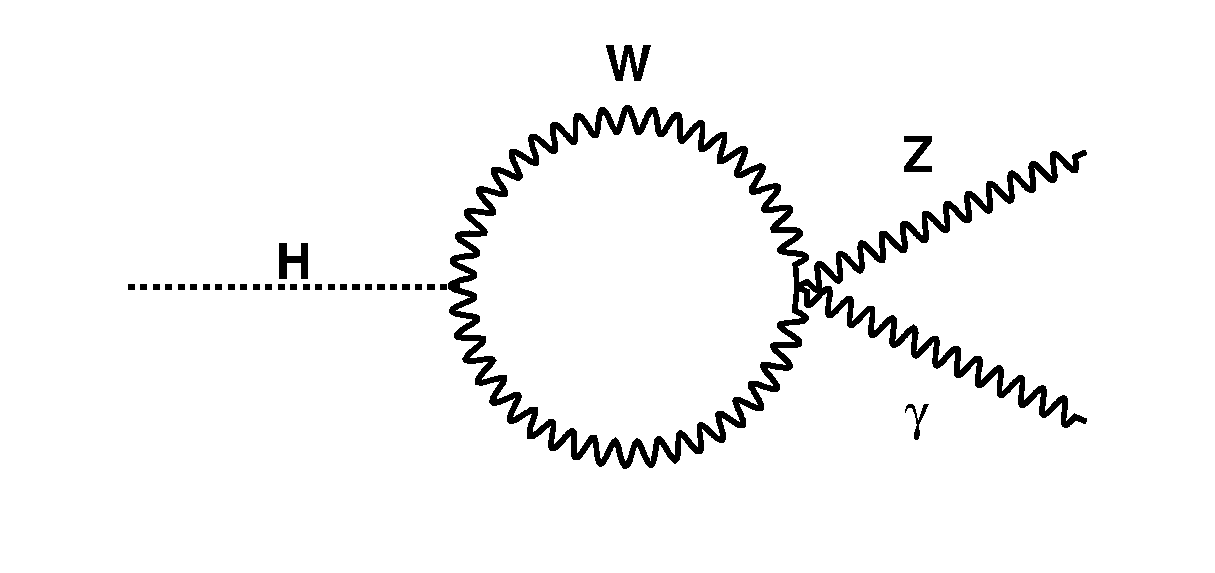
\includegraphics[width=2in]{figures/loop3}}
  \caption{Leading Feynman diagrams for the $H\rightarrow Z\gamma$
    decay in the Standard Model. Note that in the case of the fermion
    loop, top quarks dominate.} 
  \label{fig:feynman}
  \end{center}
\end{figure}

% There are many ways to analyze the dynamics of a particle classically; however,
% the one most suited for studying the symmetries of a system is Lagrangian Mechanics.
% The study of such a systems begins by defining a Lagrangian function as
% \begin{equation}
%     L(q, \dot q) = T - U 
% \end{equation}
% where $T$ and $U$ are the particle's kinetic and potential energy respectively, 
% so that the Lagrangian is a function of the particle's coordinates and velocities. 
% The mathematics behind the Standard Model is formulated in terms of the Langrian
% approach to mechanics; however, a minor detail arises because the Standard Model
% describes fields not particles.
% 
% The Standard Model is a Quantum Field Theory meaning that it is not interested in
% describing particles, which are localized entities, but in describing the
% dynamics of fields, which occupy some extended region of space. For example the
% electromagnetic field $\mathbf{E}$ is a vector vield that is described 
% by three component functions that can change throughout space and time: 
% $\mathbf{E}(\phi_i) = (\,\phi_x(x,y,z,t), \phi_y(x,y,z,t), \phi_z(x,y,z,t)\,)$. 
% As such the Lagrangians contained in the Standard Model are functions of these
% fields and their derivative.
% 
% As an introduction to how these mathematical formalism works let's consider the
% Lagrangian descibing QED:
% \begin{equation}
% \mathcal{L} = \frac{-1}{16\pi}\left(\partial^{\mu} A^{\nu} - \partial^{\nu}A^{\mu}\right) = 
% \frac{-1}{16\pi} F^{\mu\nu}F_{\mu\nu}.
% \end{equation}
% were $A^{\mu} = (\phi, \mathbf{A})$ is the electomagnetic potential.


\input{sec_atlas}
\label{sec:atlas}

\section{Signal and Background Simulation Samples}

\label{sec:sigbkg}

\section{Event Selection}
\label{sec:event}

Although the ATLAS detector measured billions of proton-proton collisions in 2011
and 2012 only a small fraction contain \HToZg decays. Therefore, an efficient
means of identifying these events using the tracking, particle identification, 
energy, and momentum information provided by the ATLAS detector is developed.
This section begins with a summary of the data samples used in this analysis
as well as any pre-analysis kinematic requirements applied to the data.
Next the algorithms used to reconstruct and identify the final state muons,
electrons, and photons from the crude information provided by the ATLAS detector
are outlined. Finally, the criteria used to interpolate back to the $Z$ and 
Higgs bosons is summarized. 

\subsection{Data Samples}
To ensure that the analyzed data is of high quality, events in which the ATLAS
detector is not fully operational, or shows data quality problems are excluded.
The resulting integrated luminosity after the trigger and data quality 
requirements corresponds to 20.7 \ifb (4.6 \ifb), with a relative uncertainty
of 3.6\% (1.8\%) at $\rts =$ 8 TeV ($\rts =$ 7 TeV) 
\cite{Aad:2011dr, Aad:2013ucp}.
Unless explicitly specified, the selection criteria
at $\rts = 8 \TeV$ and $\rts = 7 \TeV$ are identical. Values quoted in parentheses
correspond to the $\rts = 7 \TeV$ run period.


The data quality is determined by requiring the event to belong to a good runs list 
(GRL) generated by the ATLAS HSG2 group, and rejecting events with measurement 
errors in the lAr calorimeter, measurement errors in tile calorimeter, or are 
determined to be corrupt. 
The fraction of events removed in data by the GRL requirement
is around 7\% in 2011 data and 4-5\% in 2012 data. In addition, the fraction of
events with lAr, tile, or corrupt events is 0.3\% in 2011 and 0.5-0.6\% in 2012 
\cite{Abreu:1500529}.

In order to remain as unbiased as possible, the data is selected using the lowest
threshold, unprescaled single-lepton and di-lepton triggers. For the
single-muon trigger the transverse momentum, \pt, threshold is 24 (18) GeV, while
for the single-electron trigger the transverse energy, \et, threshold is 24 (20) GeV.
For the di-muon triggers, the thresholds are \pt $>$ 13 (10) GeV for each muon, while
for the di-electron triggers the thresholds are \et $>$ 12 GeV for each electron.
An asymmetric di-muon trigger is used at $\rts = 8 \TeV$ that requires one muon with 
a \pt $>$ 18 GeV and another with \pt $>$ 8 GeV. 
The trigger efficiency for signal
events passing the selection described is around 99\% for events in which the
$Z$ boson decays into $ee$ (the $ee\gamma$ channel) and 92\% for events where
the $Z$ boson decays to $\mu\mu$ pairs (the $\mu\mu\gamma$ channel). The lower
efficiency of the muon trigger is due to the reduced geometric acceptance of the muon
trigger system in the $|\eta| < 1.05$ region \cite{ATLAS-CONF-2013-009}.

In addition to an event trigger, the datasets are pre-filtered to 
reduce their size, allowing for a reasonable computing time.
The skims used were originally developed for data-driven photon identification
efficiency measurements using radiative $Z \to \ell\ell\gamma$ decays and
are based on loose kinematic and quality selections on the leptons. The
skims require at least one primary vertex with three associated tracks,
a lepton transverse momenta and photon transverse energy greater than 10 GeV,
{\tt loose++} electron identificaiton or {\tt loose} muon identification for
the lepton candidates, and at least one same flavor lepton pair with invariant mass
greater than 10 GeV. These filters retain roughly 3 - 4\% of the original events
\footnote{See this wiki for more details 
{\tt https://twiki.cern.ch/twiki/bin/viewauth/AtlasProtected/RadiativeZDAODs}.}.

\subsection{Primary Vertex Definition}
Events that pass the selection described below always have at least one
reconstructed primary vertex. These primary vertices are determined from fits
to tracks reconstructed in the inner detector and consistent with a common origin.
The interactions produced at the LHC are a result of collisions between the quarks
and gluons that make up the protons in the beams. These QCD processes are
classified as hard or soft depending on the amount of momentum transferred 
between the interacting particles. Of the roughly 20 proton-proton interactions
that occur during each bunch crossing, almost all of them are soft QCD processes.
This means there is very low momentum transfer and they mostly consist of glancing 
collisions between the quarks. However, the QCD process that produces a Higgs boson 
(gluon-gluon fusion) is a hard interaction with high momentum transfer.
In order to ensure that the primary vertex originated from the original hard 
interaction, the vertex is chosen with the largest sum of the 
squared transverse momenta of the tracks associated to it.

\subsection{Final State Particle Reconstruction and Selection}
Recall that two oppositely charged leptons ($\ell = e, \mu$) and a photon ($\gamma$)
make up the final state particles of a \HToZg event. This section
contains information regarding the reconstruction and identification of these 
particles from their energy deposition in the calorimeters and their tracking
information provided by the inner detector and the muon spectrometer.
In addition, the kinematic requirements enforced in order to select $\ell\ell\gamma$
triples originating from a Higgs decay are outlined. The sections proceed
as follows: muons, electrons, then photons.

\subsubsection*{Muon Reconstruction and Identification}
In ATLAS four kinds of muon candidates are distinguished depending on the
way they are reconstructed: stand-alone muons, combined muons, segment tagged muons,
and calorimeter tagged muons\cite{ATLAS-CONF-2010-064}.
\begin{itemize}
    \item \textbf{Stand-alone muons (SA):} SA muons are reconstructed entirely from
    tracking information provided by the muon spectrometer. The muons momentum
    is extrapolated back to the interaction point while taking into account the
    deviating effects from multiple coulomb scattering and energy loss in the 
    transversed material. SA muons utilize the extended coverage of the muon 
    spectrometer 
    and are used in the forward region ($2.5 < |\eta| < 2.7$) outside the 
    inner detector's coverage. Their use increases the overall acceptance 
    of the analysis. To increase the purity of these tracks, hits
    in all three muon spectrometer components where they are expected to pass
    are required.

    \item \textbf{Combined muons (CB):} The momentum information recorded by
    the MS is combined with the momentum measured in the inner detector. The
    muon trajectory in the inner detector also provides information about the 
    impact parameter of the muon trajectory with respect to the primary vertex.

    \item \textbf{Segment tagged muon (ST):} A trajectory in the inner detector
    is identified as a muon if the trajectory extrapolated to the muon spectrometer
    can be associated with straight track segments in the precision muon chambers,
    i.e the muon drift tubes or the cathode strip chambers.

    \item \textbf{Calorimeter tagged muon (CT):} A trajectory in the inner detector
    is identified as a muon if the associated energy deposition in the calorimeters
    is compatible with the hypothesis of a minimizing ionizing particle\footnote{
    A minimum ionizing particle (MIP) is defined as a particle whose rate 
    of mean energy loss through matter is close to the minimum. 
    The EM calorimeter is designed such that muons are MIPs, so this information
    can be used to identify muons in the calorimeter.}.
    CT muons are used to cover the region
    $|\eta| \approx 0$ which is not equipped with muon chambers. The purity
    of these muons is further increased by requiring their
    transverse momentum exceed 15 GeV.
\end{itemize}
In this analysis, CB, ST or SA muons identified with the STACO reconstruction 
algorithm as well as CT muons are used.

\subsubsection*{Muon Selection}
In the center of the barrel region ($|\eta| < 0.1$), which lacks muon spectrometer
coverage, calorimeter tagged muons with $\pt > 15 \GeV$ are used. All muon candidates
identified as muons using the information from the muon spectrometer (combined,
stand-alone, segment tagged) are required  to have a transverse momentum 
$\pt > 10 \GeV$. Each of these muons is used in the region where they have
the highest purity: combined and stand-alone muons are required to have $|\eta| < 2.7$
, and stand-alone muons are required to have $2.5 < |\eta| < 2.7$. The inner
detector tracks associated to muons that are identified inside the ID acceptance are
required to have a minimum number of associated hits in each of the ID sub-detectors
(to ensure good track reconstruction). A summary of the inner-detector hit 
requirements is summarized in \refT{tab:muonidhits}. In addition, the inner
detector tracks are required to have transverse (longitudinal) impact parameter
$d_0$ ($z_0$) with respect to the primary vertex, smaller than 1 mm (10 mm).

\begin{table}[hbt]
   \centering
   \begin{tabular}{cc}
      \hline
      \hline
      \multicolumn{2}{c}{2012} \\
      \hline
      ID Si hit requirement & expectBLayerHit=false or numberOfBLayerHits $\geq$ 1 \\
                            & No. of pixel hits $+$ No. of crossed dead pixel sensors $ > $ 0 \\
                            & No. of SCT hits $+$ No. of crossed dead SCT sensors $ > $ 4 \\
                            & No. of pixel holes $+$ No. of SCT holes $ < $ 3 \\
      TRT hit requirements: $0.1 < |\eta|\le1.9$& Hits + Outliers $>$ 5 \& $\frac{\rm{Outliers}}{\rm{Hits + outliers}}<0.9 $\\
TRT hit requirements: $|\eta| < 0.1 $ or $|\eta|\geq1.9$ & if (Hits + Outliers $>$ 5):  $\frac{\rm{Outliers}}{\rm{Hits + outliers}} <0.9 $\\
\hline
\hline
      \multicolumn{2}{c}{2011} \\
      \hline
      ID Si hit requirement & expectBLayerHit=false or numberOfBLayerHits $\geq$ 1 \\
                            & No. of pixel hits $+$ No. of crossed dead pixel sensors $ > $ 1 \\
                            & No. of SCT hits $+$ No. of crossed dead SCT sensors $ > $ 5 \\
                            & No. of pixel holes $+$ No. of SCT holes $ < $ 3 \\
      TRT hit requirements: $|\eta|<1.9$& Hits + Outliers $>$ 5 \& $\frac{\rm{Outliers}}{\rm{Hits + outliers}}<0.9 $\\
TRT hit requirements: $|\eta|\geq1.9$ & if (Hits + Outliers $>$ 5):  $\frac{\rm{Outliers}}{\rm{Hits + outliers}} <0.9 $\\
\hline
\hline
  \end{tabular}
   \caption{List of Inner Detector hit requirements for the muon
     tracks reconstructed in the ID.\label{tab:IDhits}}
   \label{tab:muonidhits}
\end{table}

\subsubsection*{Electron and Photon Reconstruction}
The electron and photon reconstruction are seeded from clusters of energy deposited
in the electromagnetic calorimeter. The reconstruction is designed to separate 
electrons, unconverted photons, and photons which have converted in the detector
material to electron-positron pairs. The clusters are matched to tracks and to 
conversion vertex candidates, which have 
been reconstructed in the inner detector and extrapolated to the second layer of
the calorimeter \cite{ATL-PHYS-PUB-2011-007}.
Electromagnetic clusters with a matching track in the inner-detector are classified
as electrons. The interaction of photons with the ATLAS detector can be
classified into two main categories: converted and unconverted photons. Converted
photons are classified by the presence of at least one ID track matching an
electromagnetic cluster originating from a vertex in the tracking volume. Clusters
without a matching track are classified as unconverted photons. Tracks matched
to electron candidates (and, for 8 TeV data, from photon conversions) and having
enough associated hits in the silicon detectors are fitted using a Gaussian-Sum
Filter, which accounts for bremsstrahlung energy loss \cite{ATLAS-CONF-2012-047}.
The energies of the clusters are calibrated, separately for electrons, converted
and unconverted photon candidates, to account for energy losses upstream of the 
calorimeter and for energy leakage outside of the cluster. In data, the calibration 
is refined by applying $\eta$-dependent correction factors, which are of the order
of $\pm 1\%$, determined from data-to-MC comparisons of the Z boson mass peak in
$\Zboson \to \epem$ events \cite{Aad:2011mk}. 
In addition, the energy measurement of converted
photons is improved with corrections, evaluated as a function of the conversion
radius (i.e. the distance from the beam-line at which the photon converts into an
\epem pair) based on dedicated Monte-Carlo simulation studies.

\subsubsection*{Electron Selection}
Electron candidates are required to have a transverse energy greater than 10 GeV,
pseudorapidity $|\eta| < 2.47$, and a well-reconstructed ID track pointing to an 
electromagnetic calorimeter cluster. The cluster should satisfy a set of 
identification criteria that require the longitudinal and transverse shower
profiles to be consistent with those expected for electromagnetic showers (
{\tt loose++} in ATLAS jargon) \cite{Aad:2011mk}. The electron four-momentum is formed
using the energy measured by the electromagnetic 
calorimeter and the track azimuth
and pseudorapidity measured in the inner detector. The electron track is required
to have a hit in the $b$-layer when passing through an active $b$-layer module
(this reduces fake electron candidates from photon conversions)
and is also required to have a longitudinal impact parameter, with respect to
the primary vertex, smaller than 10 mm.

\subsubsection*{Photon Selection}
Photon candidates are required to have a transverse energy greater than 15 GeV.
In order to exploit the fine segmentation of the first layer of the electromagnetic
calorimeter to discriminate between genuine prompt photons (photons directly produced
by parton-parton collisions) and fake photons with jets, the photon candidate 
pseudorapidity must satisfy $\abseta < 1.37$ or $1.52 < \abseta < 2.37$. The
photon four-momentum is formed using the energy measured by the calorimeter in the
direction determined by the nominal interaction point and the energy-weighted
barycenter of all cluster cells in the second layer of the calorimeter. Photons
reconstructed near regions of the calorimeter affected by read-out or high-voltage 
failures are not accepted. The identification of photons is performed through a
cut-based selection based on shower shapes measured in the first two longitudinal
layers of the electromagnetic calorimeter and on the leakage in the hadronic
calorimeter. To further suppress hadronic background, an isolation requirement is 
applied. The calorimeter isolation transverse energy $E_{T}^{\text{iso}}$ is
estimated by summing the transverse energy of three-dimensional positive-energy
topological clusters reconstructed in the electromagnetic and hadronic 
calorimeters in a cone of $\Delta R = 0.4$ around the photon candidate,
where the region within $0.125 \times 0.175$ in $\eta \times \phi$ around the
photon barycenter is excluded. The isolation energy is corrected by subtracting
the estimated contributions from leakage of the photon energy outside of the
excluded region and, using the technique described in 
Refs. \cite{Cacciari:2008gn, Cacciari:2009dp},
from the underlying event and additional $pp$ interactions. Photon candidates
are required to have an isolation transverse energy less than 4 GeV.

\subsubsection*{Overlap Removal}
An overlap removal between the electrons and muons that pass all selection
criteria and share the same inner detector track within a cone of $\Delta R < 0.02$
is performed: if the muon is identified by the MS, then the electron candidate is 
discarded, otherwise the muon candidate is rejected. Photon candidates that are
within $\Delta R < 0.3$ of a selected electron or muon candidate are also rejected,
thus suppressing background from final state radiation (FSR) $Z+\gamma$ events.

\subsection{$Z(\ell\ell)$ Reconstruction and Selection}
\subsection{$H(Z\gamma)$ Reconstruction and Selection}

\label{sec:event}

\section{Data-driven Background Estimation}
\label{sec:compare}

In this analysis the background composition is not used to determine the amount of
expected background, which is directly fitted to the data mass spectrum, but is
needed to optimize the background modeling used in the signal extraction. As outlined
in \refS{sec:event} the main backgrounds in the \HToZg search originate
from SM $Z+\gamma$ and $Z+\text{jets}$ events, with 
small contributions from $t \bar t$ and $WZ$ events.
After the full selection the relative contributions from the different backgrounds
to the selected data are 82\%, 17\%, and 1\% for $Z+\gamma$, $Z+\text{jets}$ and
$t\bar t$, respectively.

\subsection{The two-dimensional sideband (ABCD) method}
In this section a data-driven estimation of the background composition is
performed. The data-driven estimation is based on the fact that after subtracting
the $t \bar t$ and $WZ$ contributions (the electroweak background), 
the sample is composed of two categories
of events that can be discriminated by looking at the properties of the 
photon candidate. In $Z+\gamma$ events, the photon candidate is a 
prompt photon\footnote{A prompt photon is defined experimentally as an
isolated, high $\pt$ photon.},
which gives rise to a narrow energy cluster in the electromagnetic calorimeter and
is usually isolated from hadronic activity. In contrast, photons in $Z+\text{jets}$
events are the result of the decay of a neutral meson (typically a $\pi^0$)
carrying a large fraction of the initial parton energy and giving rise to an
energy cluster in the electromagnetic calorimeter which is usually energetic,
has non-negligible leakage in the hadronic calorimeter, and is not isolated from
hadronic activity, as the other particles in the same jet deposit energy in the
calorimeters near the photon candidate. Therefore, we use photon identification
and isolation variables to discriminate on a statistical basis $Z+\gamma$ and
$Z+\text{jet}$ events in data. A comparison of an actual photon shower shape
with a similar shower caused by a $\pi^0$ in the ATLAS detector are presented
in \refF{fig:photonshowers}. This technique was developed and utilized
by ATLAS in the measurement of the Standard Model prompt photon production
cross section \cite{Aad:2010sp}. 

\begin{figure}[htbp]
   \centering 

    \begin{subfigure}[b]{0.45\textwidth}
        \centering
        \includegraphics[scale=0.5, angle=0]{./figures/nicephoton}
        \caption{}
        \label{fig:nicephoton}
    \end{subfigure}
    \quad 
    \begin{subfigure}[b]{0.45\textwidth}
        \centering
        \includegraphics[scale=0.5, angle=0]{./figures/fakephoton}
        \caption{}
        \label{fig:fakephoton}
    \end{subfigure}
    \caption{A nice photon candidate (Fig.~\ref{fig:nicephoton}) and a fake photon 
    (Fig.~\ref{fig:fakephoton}) candidate as seen by the ATLAS electromagnetic
    calorimeter. Notice that the photon in \refF{fig:nicephoton} is well isolated
    from other particle showers, while the photon in \refF{fig:fakephoton} is not.}
    \label{fig:photonshowers}
\end{figure}

In the two-dimensional plane formed by the photon transverse energy and
the photon tight identification variable, we define four regions:
\begin{itemize}
 \item Tight and isolated region (\textbf{signal region A}):\\
 isolated ($\et^{\text{iso($\Delta R < 0.4$)}} < 4 \GeV$) photon candidates 
 passing the tight selection criteria (mostly $Z+\gamma$ events). 
%
 \item Tight but not-isolated region (\textbf{control region B}):\\
 tight, non-isolated ($\et^{\text{iso($\Delta R < 0.4$)}} > 5 \GeV$) 
 photon candidates (non-isolated $Z+\text{jets}$ background).
%
 \item Not-tight and isolated region (\textbf{control region C}): \\
 candidates that have an isolated ($\et^{\text{iso($\Delta R < 0.4$)}} < 4 \GeV$)
 photon passing the not-tight selection (non-identified $Z+\text{jets}$ background). 
%
 \item Not-tight and not-isolated region (\textbf{control region D}): \\
 contains non-isolated ($\et^{\text{iso($\Delta R < 0.4$)}} > 5 \GeV$), 
 non-tight photon candidates ($Z+\text{jets}$ background).
\end{itemize}

\begin{figure}[!hbpt]
  \centering
  \includegraphics[scale=0.60]{figures/2dsketch.eps}
  \caption{Illustration of the two-dimensional plane, defined	
      by means of the isolation and a subset of the photon
      identification (ID) variables, from the observed yields $N_{B},
      N_{C}$ and $N_{D}$ in the three control regions, the background
    yield in the signal region were the observed total signal yield is
    $N_{A}$}
\label{fig::2dsketch}
\end{figure}

The 2D-sideband method is based on the following two assumptions: 
\begin{enumerate}
\item The signal contamination in the three background control regions (B, C, and D)
is small. This implies that all reconstructed photons falling in
one of these regions are coming from a background event. In particular, the
fraction of events coming from jet-faking events $N^{Z\text{jet}}$ can be
extracted by subtracting the contribution from electroweak backgrounds 
\New{} (estimated from Monte Carlo) from the total number of
observed events in each of these three regions: $N_A = \Nzg{A} + \Nzj{A} + \New{A}$
for the signal region and $N_K = \Nzj{K} + \New{K}$ ($K \in \{B, C, D\}$) 
for each control region.
%
\item The ratio of isolated to non-isolated background candidates from the jet-fake
in the not-tight bins $\left(\frac{\Nzj{D}}{\Nzj{C}}\right)$
is equal to the same ratio computed in the tight bins
$\left(\frac{\Nzj{B}}{\Nzj{A}}\right)$.
\end{enumerate}
These statements imply that the $Z+\text{jets}$ background in region A can
be calculated as follows:
\begin{equation}
    \Nzj{A} = (N_B - \New{B})\frac{(N_C - \New{C})}{(N_D - \New{D})}.
\end{equation}
Thus, the $Z+\gamma$ yield \Nzg{A} in region A is estimated from the number
of events in the data in the four regions as
\begin{equation}
   \Nzg{A} = (N_A - \New{A}) - (N_B - \New{B})\frac{(N_C - \New{C})}{(N_D - \New{D})}.
\end{equation}
where \New{} is estimated from electroweak background Monte Carlo simulations.

However, one must correct for the fact that the number of signal events in the
background control regions is always positive and non-zero by defining the
\emph{signal leakage fractions} $c_K = N_K^{Z\gamma\text{MC}}/N_A^{Z\gamma\text{MC}}$
that can be extracted from simulated $Z+\gamma$ samples. In addition,
there are correlations between the photon isolation variable and the
photon identification quantities that are corrected by a correlation 
coefficient
\begin{equation} 
    R^{Z\text{jetsMC}} = \frac{\Nzjmc{A} \Nzjmc{D}}{\Nzjmc{B} \Nzjmc{C}}
\end{equation}
obtained from high statistics $Z+\text{jets}$ simulated events, after removing
- using the truth information - the contributions from $Z+\gamma$ processes.
The final result for the signal yield is then
\begin{equation}
   \Nzg{A} = (N_A - \New{A}) - (N_B - \New{B} - c_B\Nzg{A})\frac{(N_C - \New{C} - c_C\Nzg{A})}{(N_D - \New{D} - c_D\Nzg{A})}\,R^{Z\text{jetsMC}}.
\label{eq:2destB}
\end{equation}
This is a second-order polynomial equation in $N_A^{Z\gamma}$ that only has
one physical solution, i.e. a positive solution. Finally, the $Z+\text{jets}$
background is obtained as
\begin{equation}
\Nzj{A} = N_A - \New{A} - \Nzg{A}.
\label{eq:2destA}
\end{equation}

\subsection{Data-Monte Carlo comparisons}
Following the discussion in the previous section the $Z$+jets background to
$Z\gamma$ processes are estimated using Equation~\ref{eq:2destA} and \ref{eq:2destB}.
In the following we define the purity ($P$) of $Z\gamma$ candidate samples as
\[
    P = \frac{N_A - \Nzj{A} - \New{A}}{N_A}.
\]
A summary of the different measured backgrounds as well as the purity of $Z\gamma$
events in data are calculated and summarized in \refT{tab:zgbgsummary}.
After the full selection the relative contributions from the different backgrounds
to the selected data are 82\%, 17\%, and 1\% for $Z+\gamma$, $Z+\text{jets}$ and
$t\bar t$, respectively.
In addition, a comparison between data and the simulation after scaling each 
MC background contribution to the number of events estimated in data is shown in 
\refF{fig:zgamma_mass_linear} and \ref{fig:Dm_mass_linear}. 
A good agreement between data and simulation is observed.

\begin{table}[!htbp]
\centering
\caption{
 Estimations of $Z$+jets and electroweak background events after all $H\rightarrow Z \gamma$ selection cuts in electron and muon categories for the 2012 and 2011 datasets, which have luminosities around 20.7 fb$^{-1}$ and 4.6 fb$^{-1}$, respectively. Errors in MC $t\bar{t}$, $WZ$ and extracted Data-Driven $Z\gamma$ events are only statistical.}
  \label{tab:zgbgsummary}
\begin{tabular}{ccccccc}
       \hline
%%      \textbf{background source } & $pp \rightarrow e^{+}e^{-}\gamma$  & $pp \rightarrow \mu^{+}\mu^{-}\gamma$ \\
       \textbf{background source } & $Z(e^{+}e^{-})\gamma$  & $ Z( \mu^{+}\mu^{-})\gamma$ \\
       \hline
 	  &   {\bf 8TeV} &  \\
       \hline
	   
      total observed events & 13898    &  16658 \\
       \hline
        $Z$+$jets$             & $ 2137.58 \pm 116.94 \pm 541.45  $ &  $ 2561.69 \pm 109.23  \pm 474.94 $  \\
       $t\bar t$            &  $ 63.08 \pm 2.65 $&  $ 78.58 \pm 3.08 $ \\
 	$WZ $   	     &  $ 9.55 \pm 0.66 $ &  $ 6.97 \pm 0.52 $    \\
       \hline
   extracted $Z\gamma$ events  & $ 11687.79 \pm 166.07  $ &   $ 14010.76 \pm 169.11 $  \\
       \hline
 	Purity   		&  $ 0.841 \pm 0.014 \pm 0.039 $             &  $ 0.841 \pm  0.012 \pm 0.028$    \\
       \hline	 
       \hline
 	  &   {\bf 7TeV} &  \\
       \hline

      total observed events & 1960    &  2665 \\
       \hline
        $Z$+$jets$             & $ 318.20 \pm 45.84 \pm 34.24  $ &  $ 343.25 \pm 39.88  \pm 21.04 $  \\
       $t\bar t$            &  $ 7.45 \pm 1.17 $&  $ 8.31 \pm 1.23 $ \\
        $WZ $                &  $ 5.63 \pm 0.19 $ &  $ 5.38 \pm 0.18 $    \\
       \hline
   extracted $Z\gamma$ events  & $ 1628.72 \pm 63.74  $ &   $ 2308.06 \pm 65.25 $  \\
       \hline
        Purity                  &  $ 0.831 \pm 0.037 \pm 0.017 $             &  $ 0.866 \pm  0.030 \pm 0.015$    \\
   \hline
   \hline
      

\end{tabular}
\end{table}

\begin{figure}[!htbp]
  \begin{center}
    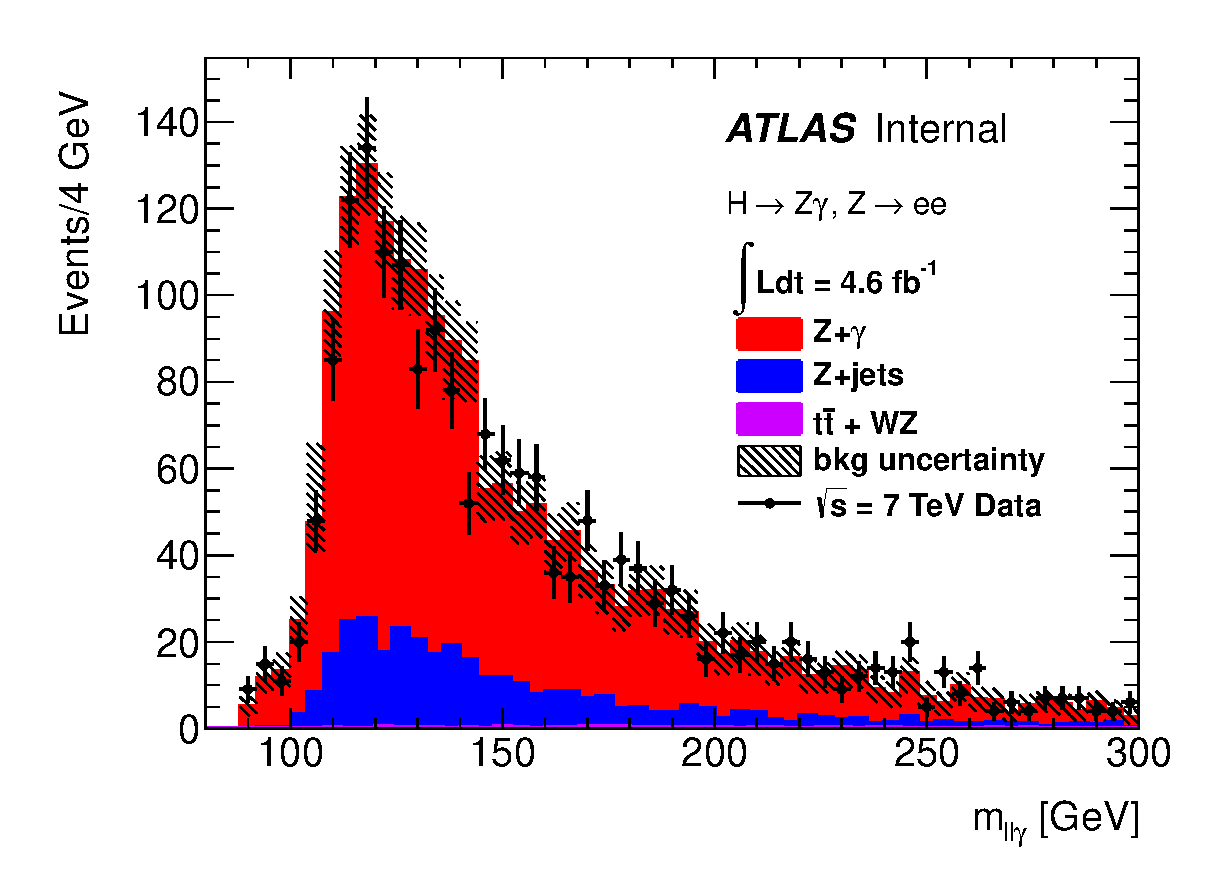
\includegraphics[width=0.49\columnwidth]{figures/bkg_decomposition_2011_e_Mllg_Z_PV_corr_linscale}
    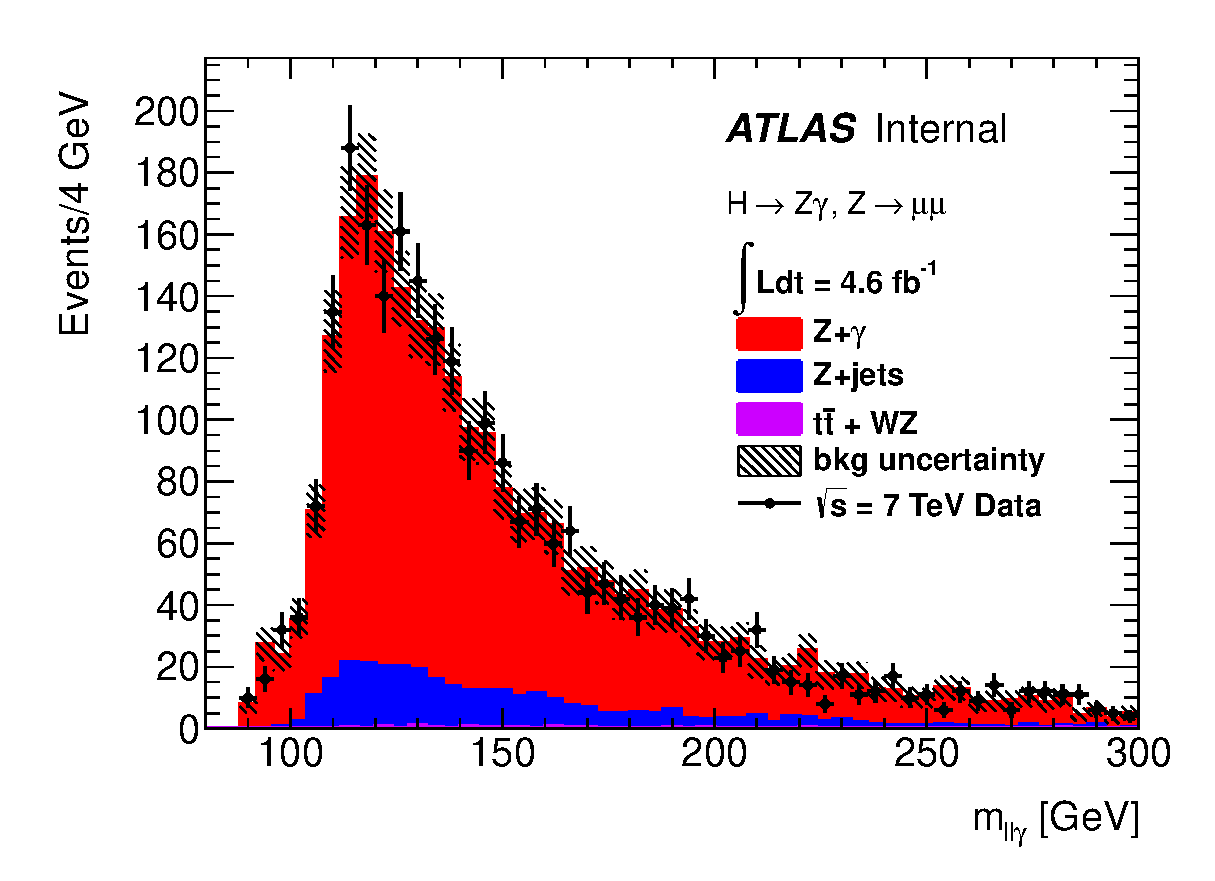
\includegraphics[width=0.49\columnwidth]{figures/bkg_decomposition_2011_mu_Mllg_Z_PV_corr_linscale}
    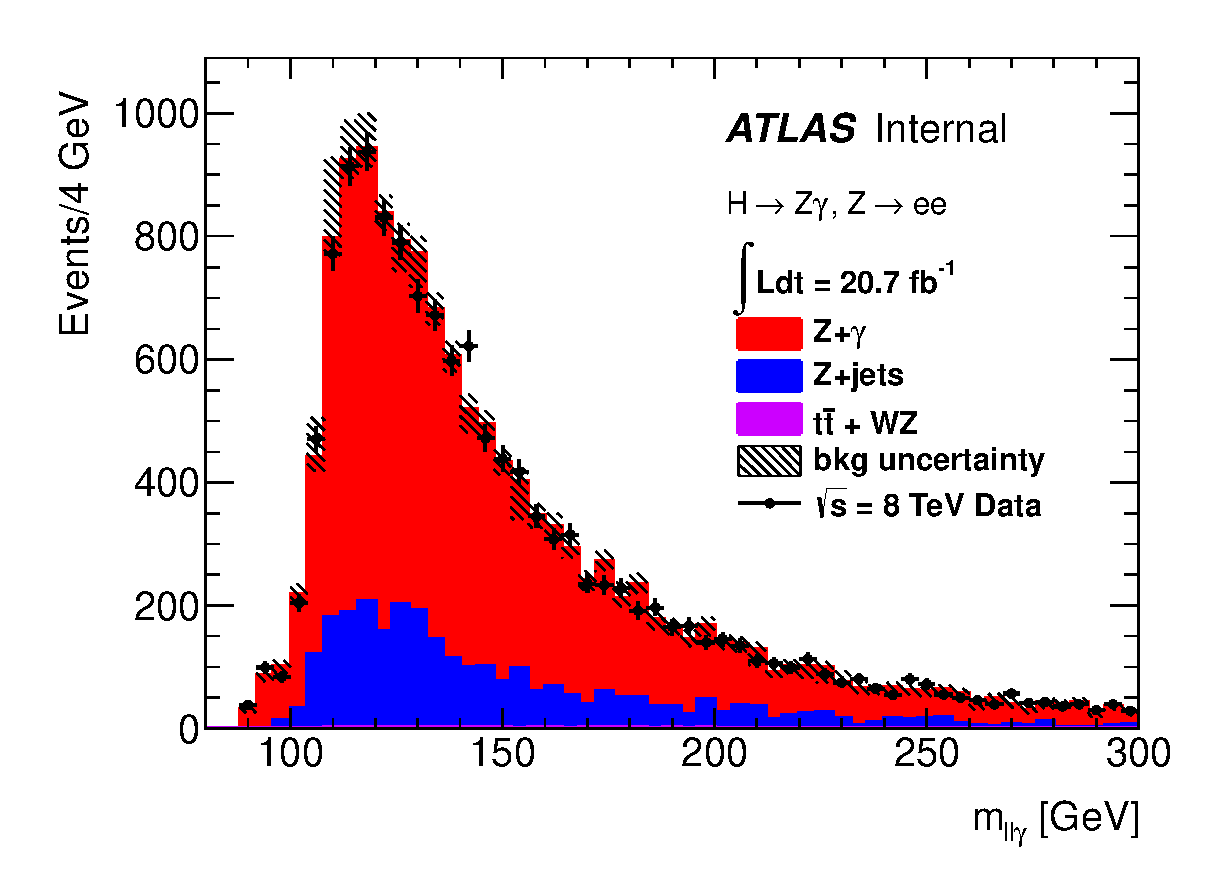
\includegraphics[width=0.49\columnwidth]{figures/bkg_decomposition_2012_e_Mllg_Z_PV_corr_linscale}
    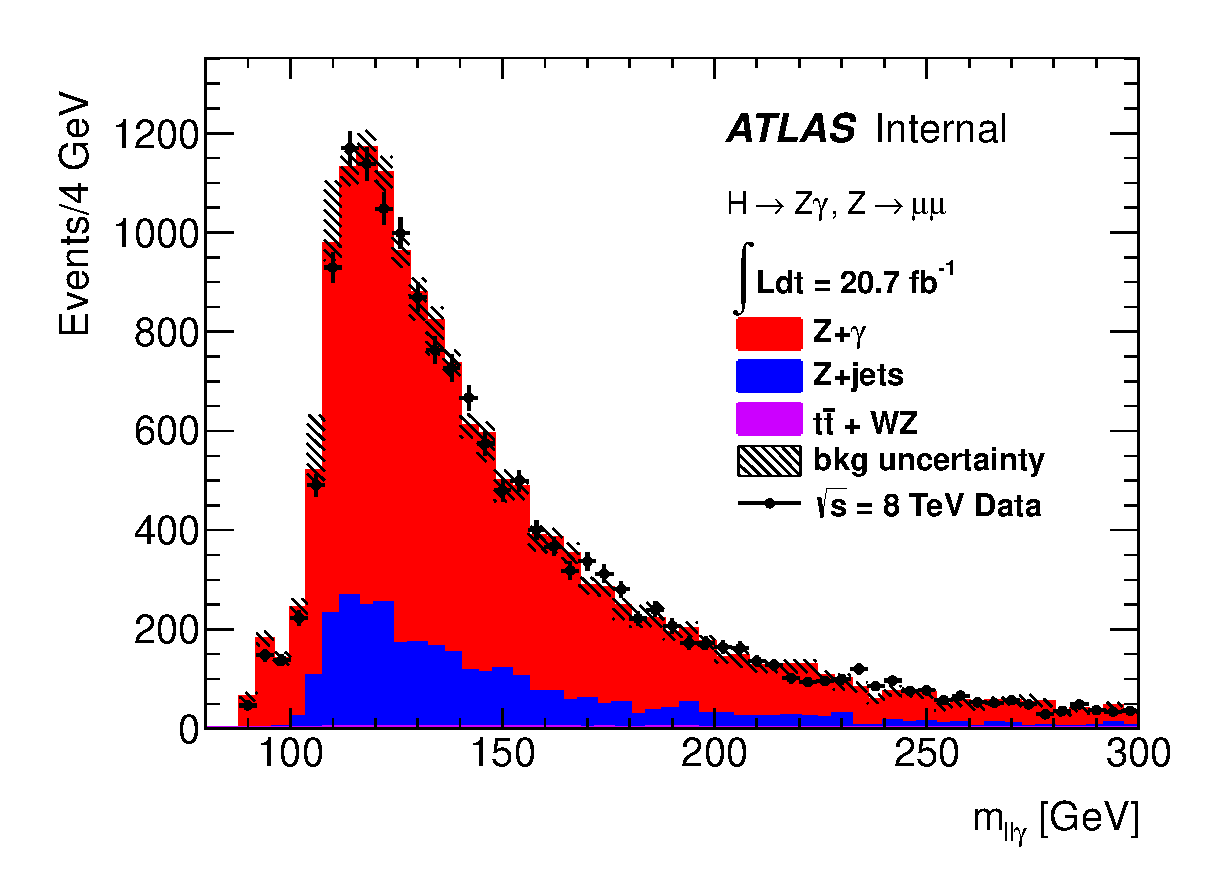
\includegraphics[width=0.49\columnwidth]{figures/bkg_decomposition_2012_mu_Mllg_Z_PV_corr_linscale}
    \caption{Three-body invariant mass $(m_{\ell\ell\gamma})$ distribution 
      of selected events in data (dots) and from the various
      background sources (histograms, from the simulation) normalized 
      to the yields determined as described in the text, 
      for $Z\to ee$ (left) and $Z\to\mu\mu$ (right) channels.
      The small peak near $m_Z$ is from residual FSR $Z$+$\gamma$ contamination.
      The background uncertainty includes statistical uncertainties and 
      systematic uncertainties from the inputs taken from the simulation, as detailed in the text.
    }
    \label{fig:zgamma_mass_linear}
  \end{center}
\end{figure}

\begin{figure}[!htbp]
  \begin{center}
    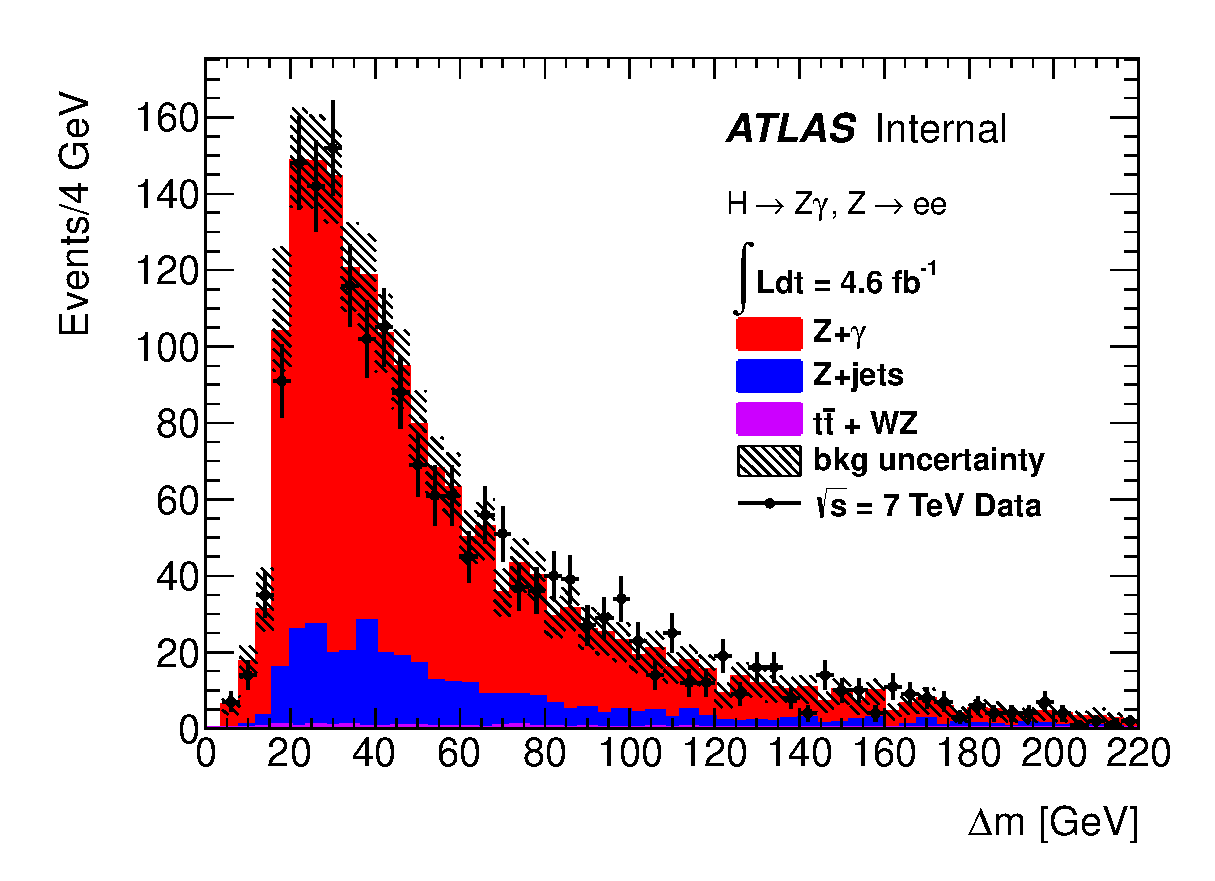
\includegraphics[width=0.49\columnwidth]{figures/bkg_decomposition_2011_e_dMllg_Z_PV_corr_linscale}
    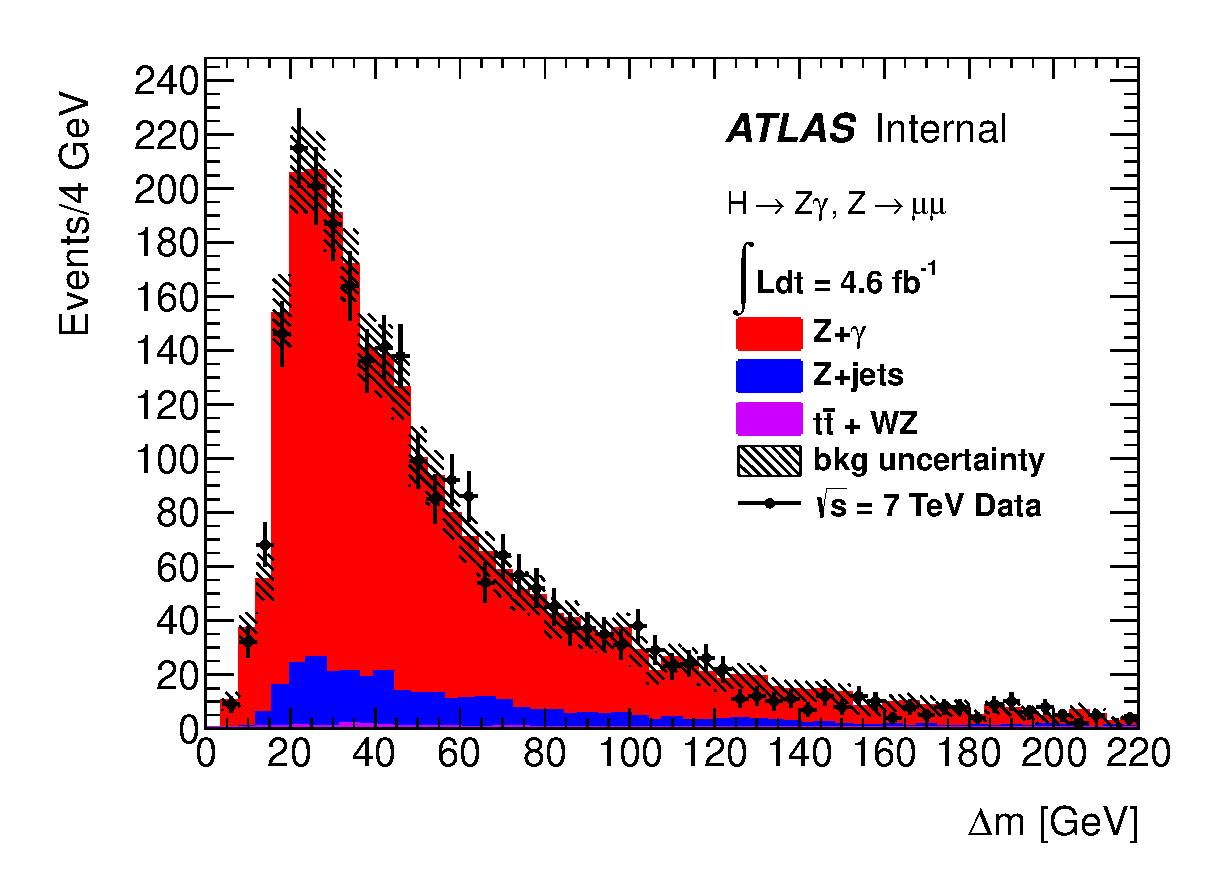
\includegraphics[width=0.49\columnwidth]{figures/bkg_decomposition_2011_mu_dMllg_Z_PV_corr_linscale}
    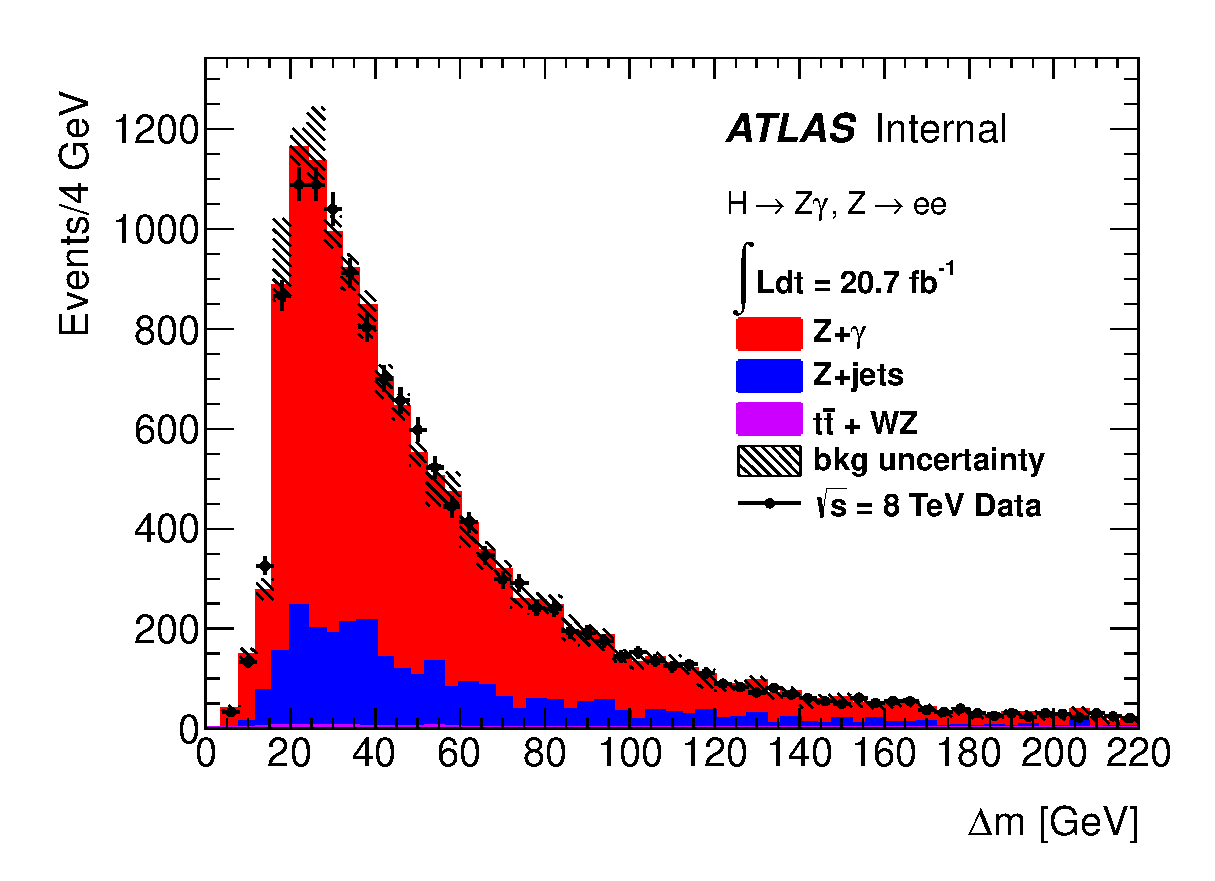
\includegraphics[width=0.49\columnwidth]{figures/bkg_decomposition_2012_e_dMllg_Z_PV_corr_linscale}
    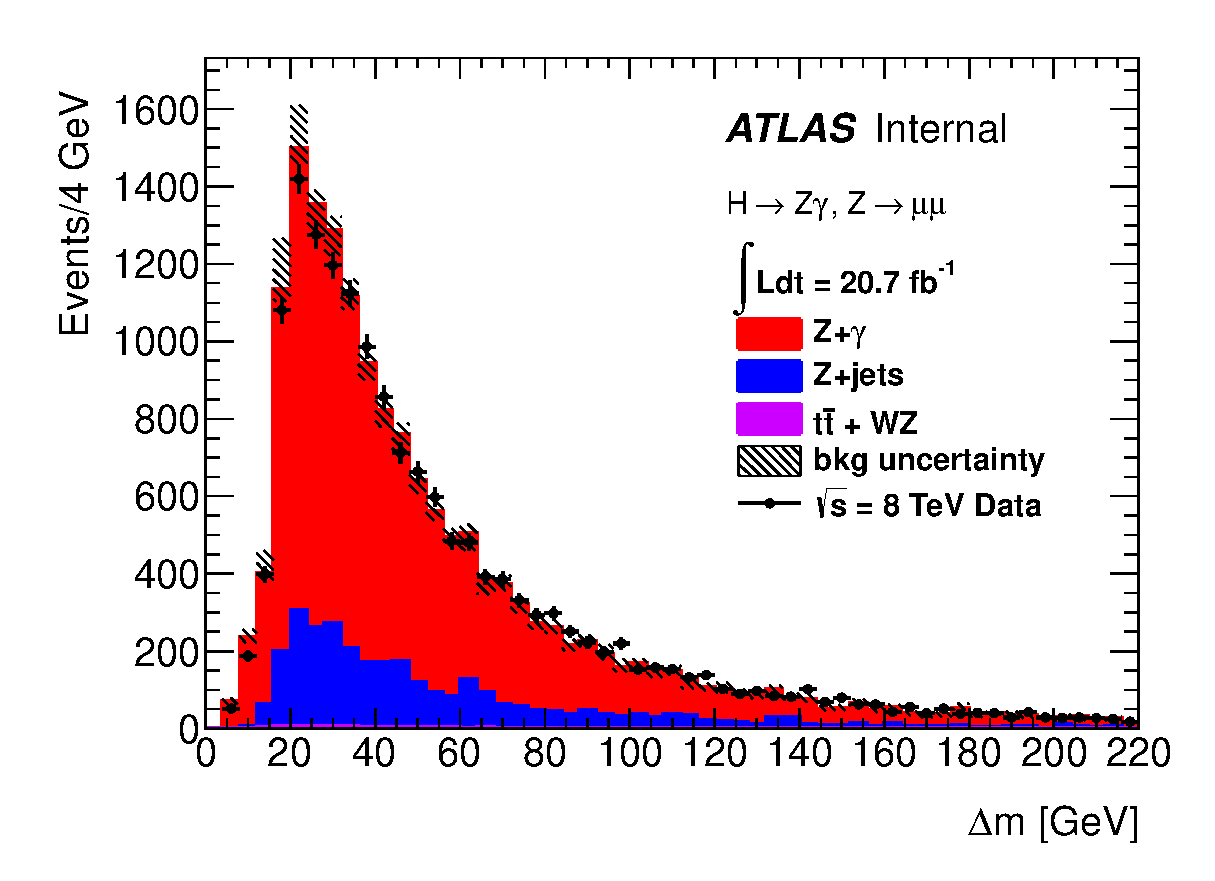
\includegraphics[width=0.49\columnwidth]{figures/bkg_decomposition_2012_mu_dMllg_Z_PV_corr_linscale}
    \caption{Distribution of the difference $\Delta m$ 
      between the final state three-body invariant mass
      $m_{\ell\ell\gamma}$ and the di-lepton invariant mass
      $m_{\ell\ell}$ for selected events in data (dots) and from
      the various background sources (histograms) normalized to the yields determined 
      as described in the text, for $Z\to ee$ (left) and $Z\to\mu\mu$ (right) channels.
      The background uncertainty includes statistical uncertainties and systematic
      uncertainties from the inputs taken from the simulation.
    }
    \label{fig:Dm_mass_linear}
  \end{center}
\end{figure}

\label{sec:compare}

\section{Signal Studies}
\label{sec:signal}
The various properties of the \HToZg signal are described in this section.
This includes a discussion of the number of signal events expected to be
observed in data (expected signal yield) followed by a description
of the template model used to describe the signal's shape in data.

\subsection{Expected Signal Yield}
An understanding of the expected signal yield follows the same calculation
described in \refS{subsec:prodproc} with an additional term that accounts
for the fact that the selection described in \refS{sec:event} will not
select all of the \HTollg events produced by the LHC. As described in
\refS{subsec:mc}, Higgs boson production and decay are simulated with
several Monte Carlo samples that are passed through a full detector simulation.
This full simulation allows for the estimation of the signal selection efficiency
and therefore the expect signal yield for a SM Higgs boson decaying to $Z\gamma$
in each decay mode ($i = gg$, VBF, etc.) via:
\[
    N_{i,\ell}(m_H) = \int L\, dt \times \sigma_i(m_H) \times 
    B_{H\to Z\gamma}(m_H) \times B_{Z\to\ell\ell} \times \epsilon_{i,\ell}(m_H)
\]
where
\begin{enumerate}
 \item $\int L\, dt$ is the integrated luminosity of the data sample,
 \item $\sigma_i(m_H)$ is the SM Higgs boson production cross section for a
 Higgs boson of mass $m_H$, in the production process $i$ ($gg$, VBF, etc.),
 \item $B_{H\to Z\gamma}$ is the branching fraction for the decay to $Z\gamma$
 of a SM Higgs boson of mass $m_H$,
 \item $B_{Z\to\ell\ell} = (3.3658 \pm 0.0023)\%$ is the $Z\to\ell\ell$ branching
 fraction \cite{PDG2012},
 \item $\epsilon_{i,\ell}(m_H)$ is the selection efficiency for \HTollg events.
\end{enumerate}
The second and third inputs are taken from
\cite{LHCHiggsCrossSectionWorkingGroup:2011ti, LHCHiggsCrossSectionWorkingGroup:2012vm}, 
while the fourth input is estimated from the ATLAS full simulation of signal events.
The expected total yield, for each lepton flavor, is then 
\[
    N_{\ell}(m_H) = \sum_i N_{i,\ell}(m_H).
\]

The signal efficiency was computed using signal Monte Carlo as
\[
    \epsilon_{i,\ell} = \frac{\sum_j w^{\text{reco}}_{j,\ell}}{\sum_k w^{\text{true}}_{k,\ell}}
\]
where
\begin{itemize}
 \item $\sum_j w^{\text{true}}_{j,\ell}$ is the sum over the events $j$ in which the
 generated $Z$ boson decays to a $\ell\ell$ pair (identified by inspecting the
 MC truth record) of the product of the `initial' weights\footnote{These are
 the Monte Carlo weights applied before the object reconstruction, i.e. pile-up
 and a $z$-vertex weight}.
 \item $\sum_k w^{\text{reco}}_{k,\ell}$ is the sum over the events $k$ in which
 the generated $Z$ boson decays to a $\ell\ell$ pair and passing the full \HTollg
 selection of the `final' weights\footnote{These are the initial weights and the 
 efficiency scale factors for the trigger, the leptons, and the photon.}.
\end{itemize}
The expected signal yields and selection efficiencies for Higgs boson masses 
between 120 and 150 GeV and for an integrated luminoisty of 20.7 \ifb (4.6 \ifb)
at $\rts = 8$ (7) TeV are shown in \refT{tab:expected_signalyields}.

\begin{table}[!htbp]
  \begin{center}
    \begin{tabular}{l|cc|cc|cc|cc}
\hline
\hline
$m_H$  & \multicolumn{2}{c|}{$Z\to ee$, 7 TeV} & \multicolumn{2}{c|}{$Z\to \mu\mu$, 7 TeV} & \multicolumn{2}{c|}{$Z\to ee$, 8 TeV} &  \multicolumn{2}{c}{$Z\to \mu\mu$, 8 TeV} \\
$[$GeV$]$ & $\varepsilon$ [\%] & $S$ & $\varepsilon$ [\%] & $S$ & $\varepsilon$ [\%] & $S$ & $\varepsilon$ [\%] & $S$ \\
\hline
120  &  17.1  &  0.6  &  22.5  &  0.7  &  21.3  &  4.0  &  25.8  &   4.9  \\
125  &  20.4  &  0.9  &  26.5  &  1.1  &  24.6  &  5.9  &  29.7  &   7.2  \\
130  &  23.0  &  1.1  &  29.9  &  1.5  &  27.3  &  7.7  &  32.8  &   9.3  \\
135  &  25.1  &  1.3  &  32.4  &  1.7  &  29.4  &  9.0  &  35.1  &  10.7  \\
140  &  26.6  &  1.4  &  34.1  &  1.8  &  30.9  &  9.5  &  36.6  &  11.3  \\
145  &  27.5  &  1.4  &  35.0  &  1.8  &  31.7  &  9.2  &  37.3  &  10.8  \\
150  &  27.9  &  1.2  &  35.1  &  1.5  &  32.0  &  8.1  &  37.2  &   9.4  \\
        \hline\hline
    \end{tabular}
  \caption{Selection efficiency ($\varepsilon$) and number of expected
    $H\to Z\gamma$ signal events ($S$),
    for Higgs boson masses between 120 and 150 GeV,
    for the two reconstructed $Z$ boson final states and
    for \lumiseventev~\ifb\ at $\sqrt{s}=7\TeV$
    and \lumieighttev~\ifb\ at $\sqrt{s}=8\TeV$.
    The relative statistical uncertainty on the quoted numbers
    is around 1\%.
    %% The relative uncertainty on the selection efficiency is
    %% around 5\%, as described in Section~\ref{sec:Systematics}.
    %% The relative uncertainty on the signal yield
    %% also includes an additional 3.6\% (1.8)\% contribution
    %% from the luminosity uncertainty in 8 (7) TeV data.
  }
  \label{tab:expected_signalyields}
  \end{center}
\end{table}


\subsection{Signal Model}
The search for the SM Higgs boson decaying to $Z\gamma$ is performed through
a fit to the distribution of an observable that discriminates between signal
and background. Two observables have been studied: the three-body invariant
mass of the final state particles, $m_{\ell\ell\gamma}$,
and the difference between the three-body
and the di-lepton invariant masses, $\dm = \mllg - \mass{\ell}$.
A choice of \dm over \mllg as the discriminating observable was made for the 
following two reasons: \dm is unaffected by the lepton energy scale uncertainties, and
it is to a large extent insensitive to the contribution from FSR in $H\to\mu\mu$
decays.

In the fit, a model for the signal and background probability density functions of
the observable under study is needed. It has been found that both observables
\mllg and \dm of signal events generated at a fix Higgs boson nominal mass are
well described by a composite model of a Crystal Ball function (CB) (a gaussian
core\footnote{A gaussian is used instead of a Lorentzian peak because of the
restricted resolution of the ATLAS detector.} 
with one exponential tail modeling energy loss due to final-state photon
radiation) \cite{Oreglia}, 
and a small wide Gaussian component (GA) modeling the distribution's outliers.
The formula for the CB function is given as follows:
\begin{displaymath}
    CB(m_H) = \left\{
            \begin{array}{lr}
            \frac{N}{\sqrt{2 \pi \sigma}} \exp\left(-\frac{(\mllg-m_H)^2}{2\sigma^2}\right), & \qquad \mathrm{for}\quad \frac{\mllg-m_H}{\sigma} > -\alpha; \\
            \frac{N}{\sqrt{2\pi\sigma}} \left(\frac{n}{|\alpha|}\right)^n \exp\left(-\frac{|\alpha|^2}{2}\right)\left(\frac{n}{|\alpha|} - |\alpha| - \frac{\mllg - m_H}{\sigma}\right)^{-n}, & \qquad \mathrm{for}\quad \frac{\mllg-m_H}{\sigma} \le -\alpha.
            \end{array}
               \right.
\end{displaymath}
where $N$ is a normalization parameter, and $m_H$ is the Higgs boson mass.

Since the parameters describing the signal model can also be a function
of the Higgs boson mass, a complete description of the signal in the whole
mass range is a function that incorporates these variations. The global
resolution model is such an analytic function of the mass given as
\[
    R(m_{\ell\ell\gamma}, \mu_{CB}, \sigma_{CB}, n_{CB}, \mu_{GA}, \sigma_{GA}) =
    f_{CB} \cdot CB\left[m_{\ell\ell\gamma}, \mu_{CB}, \alpha_{CB}, f_{CB},
    \sigma_{CB}, n_{CB}\right] + (1 - f_{CB}) \cdot
    GA\left[m_{\ell\ell\gamma}, \mu_{GA}, \sigma_{GA}\right]
\]
where $\sigma_{CB}, \mu_{CB}$ and $\sigma_{GA}, \mu_{GA}$ represent the
three-body invariant mass resolution and mean value of the core and outliers
respectively. Also $n_{CB}$ and $\alpha_{CB}$ parameterize the non-Gaussian tail, and
$f_{CB}$ is the fraction of the Crystal Ball function in the composite model.

From the available signal Monte Carlo samples at different mass points the parameters
that depend on the nominal Higgs boson mass $m_H$ were identified and the global
and mass dependent parameters were extracted from a simultaneous fit. For the mass
dependent parameters ($\mu_{CB}, \alpha_{CB}, \sigma_{CB}$) we assume a linear
dependence and fit the parameters
\[
\mu_{CB} = \mu_{CB}(m_H = 125 \GeV) + \Delta \mu_{CB}^{\text{slope}} \times \left(\mllg - 125 \GeV \right)
\]
\[
\sigma_{CB} = \sigma_{CB}(m_H = 125 \GeV) + \Delta \sigma_{CB}^{\text{slope}} \times \left(\mllg - 125 \GeV \right)
\]
\[
\alpha_{CB} = \alpha_{CB}(m_H = 125 \GeV) + \Delta \alpha_{CB}^{\text{slope}} \times \left(\mllg - 125 \GeV \right)
\]
The other parameters ($f_{CB}$, $n_{CB}$) are set at a signle global value for all
mass points. Also, the relative width of the core and outlier components are shown
to remain unchanged at all mass points, so can be set at a global value.

In total, 7 parameters per category (3 shape parameters with linear dependence of
the Higgs boson mass and 4 global parameters), are extracted from a single fit to
all available Monte Carlo samples, and are sufficient to provide a robust 
parameterization of the invariant mass probability distribution function (p.d.f.)
at any Higgs mass.

\subsection{Fits to Signal Monte Carlo Samples}

\refF{fig:signal_resolution_corrections} shows the expected mass distribution for
a Higgs boson with a mass of 125 GeV at $\rts = 8 \GeV$ 
after applying all analysis cuts and corrections.
In addition, an example of the distribution of the mass difference 
\dm for signal events passing the full selection for $m_H = 125  \GeV$ is shown in 
\refF{fig:resolution_model_example_8tev_H125}.

\begin{figure}[!htbp]
  \begin{center}
%  {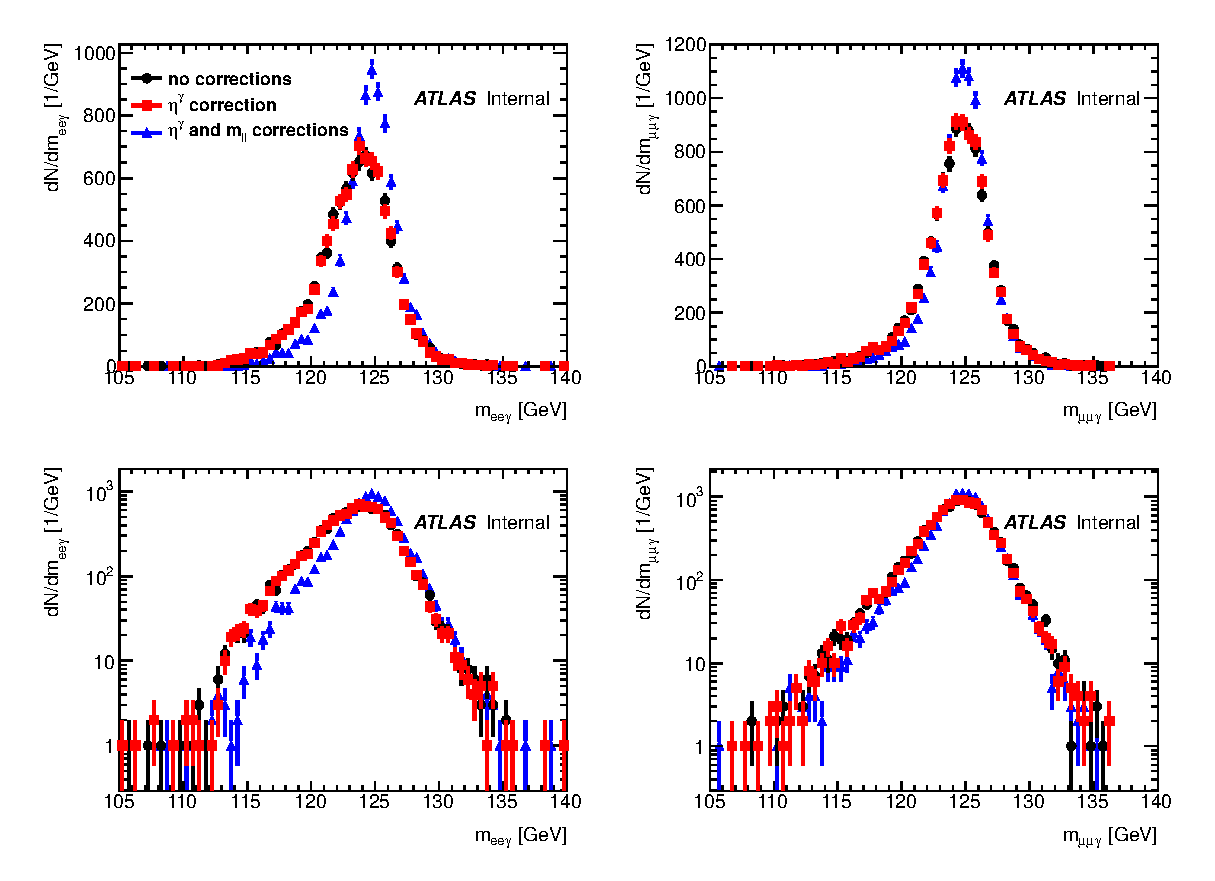
\includegraphics[width=0.99\textwidth]{figures/signal_mllg_corrections}}
{\includegraphics[width=0.48\textwidth]{figures/PlotsSuperposedResolutionCorrections_e_mc12a_Mllg}}
{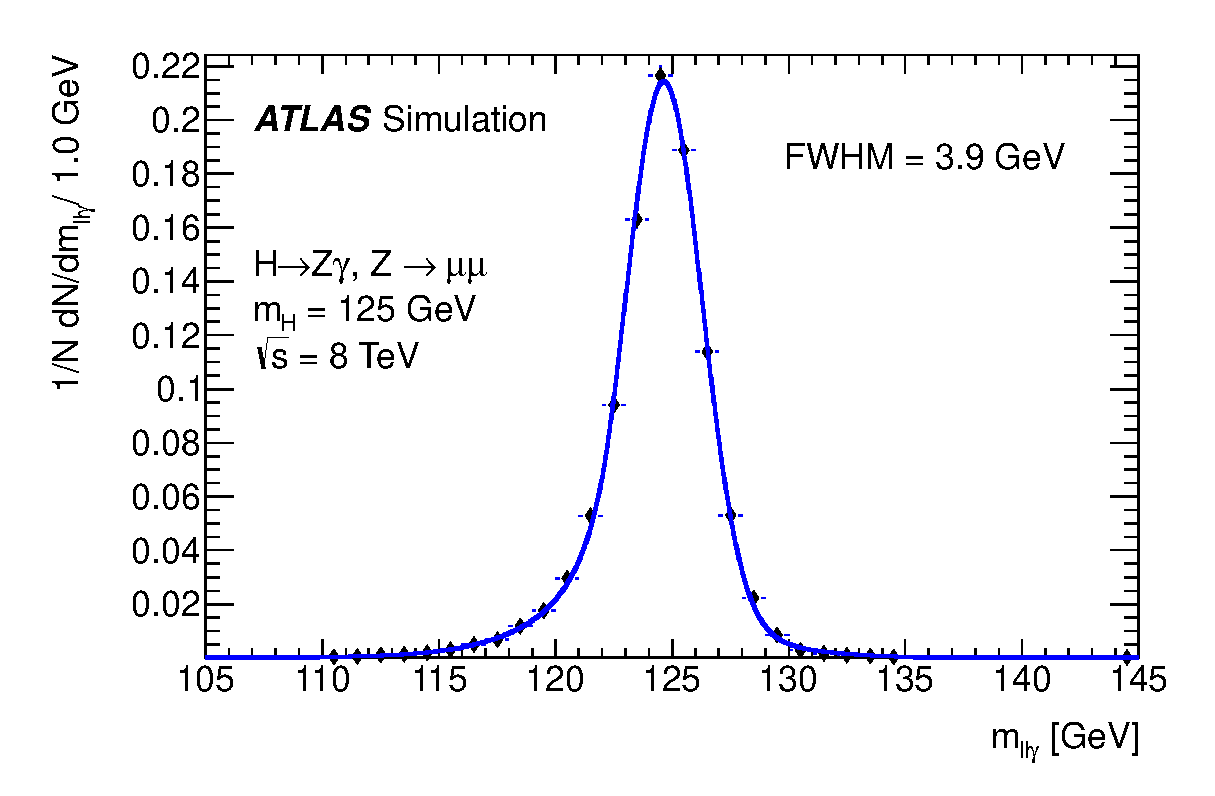
\includegraphics[width=0.48\textwidth]{figures/PlotsSuperposedResolutionCorrections_mu_mc12a_Mllg}}
\caption{Three-body invariant mass distribution for $gg\to H\to Z\gamma$
    selected events in the 8 TeV, $m_H=125$~GeV signal simulation, 
    after applying all analysis cuts and corrections. The blue solid lines 
    represent the fits to the points of the sum of a 
    Crystal Ball lineshape and a Gaussian function.
    Left: $Z\to ee$ channel, right: $Z\to\mu\mu$ channel.}
%the standard reconstruction (red circles), and after choosing the event primary vertex as the photon origin and applying the $Z$ mass constraint to the lepton four momenta (blue diamonds). The (dashed) red line and the (blue) solid line  represent the fits to the points of the sum of a Crystal Ball lineshape and a Gaussian function. Left: $Z\to ee$ channel, right: $Z\to\mu\mu$ channel.}
  \label{fig:signal_resolution_corrections}
  \end{center}
\end{figure}

\begin{figure}[!htbp]
  \begin{center}
  {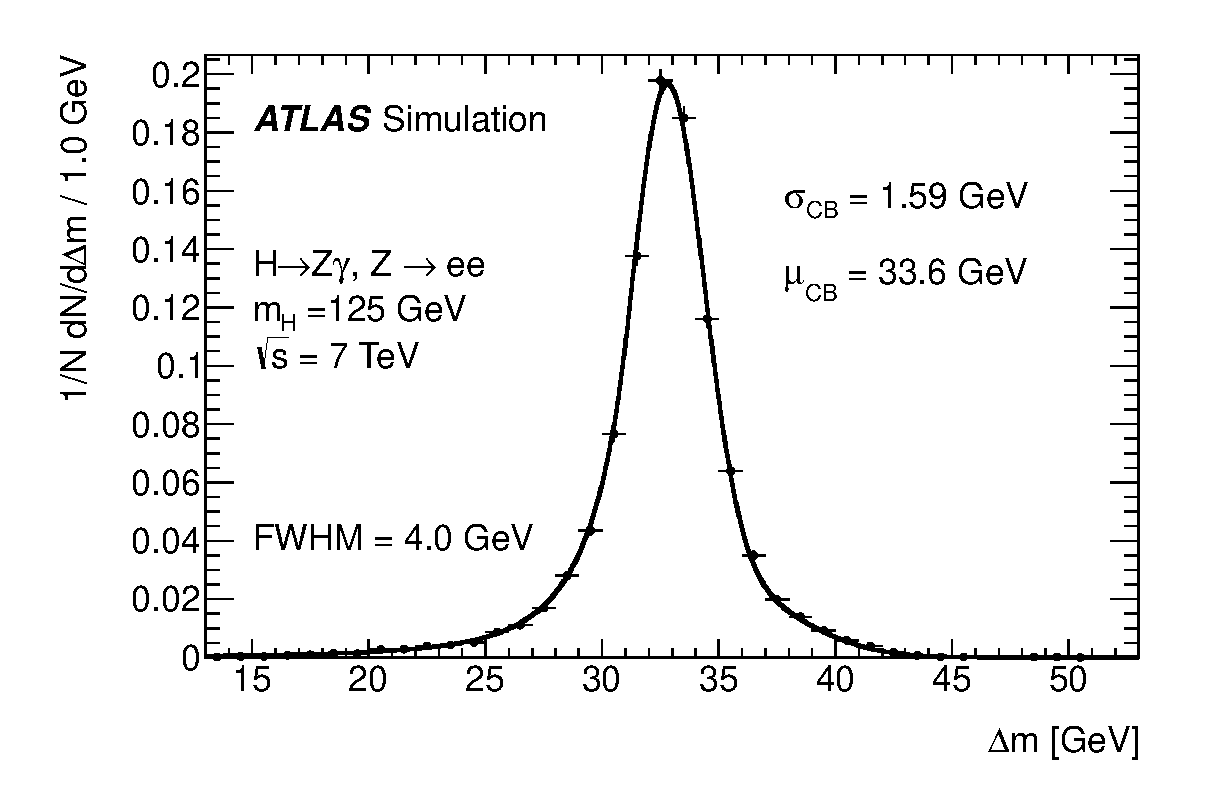
\includegraphics[width=0.46\textwidth]{figures/linPlot_125_EtaZgamma_Cat0_all_e_mc11c_mDif}}
  {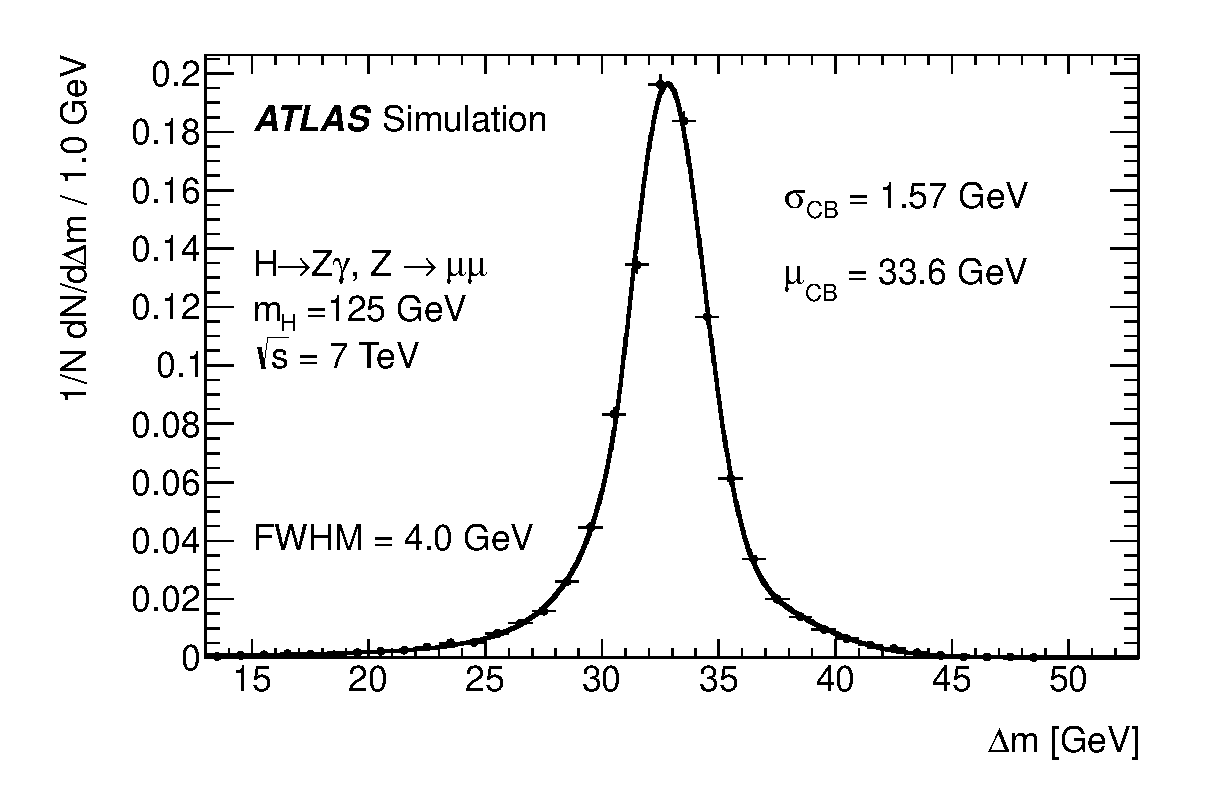
\includegraphics[width=0.46\textwidth]{figures/linPlot_125_EtaZgamma_Cat0_all_mu_mc11c_mDif}}
  {\includegraphics[width=0.46\textwidth]{figures/linPlot_125_EtaZgamma_Cat0_all_e_mc12a_mDif}}
  {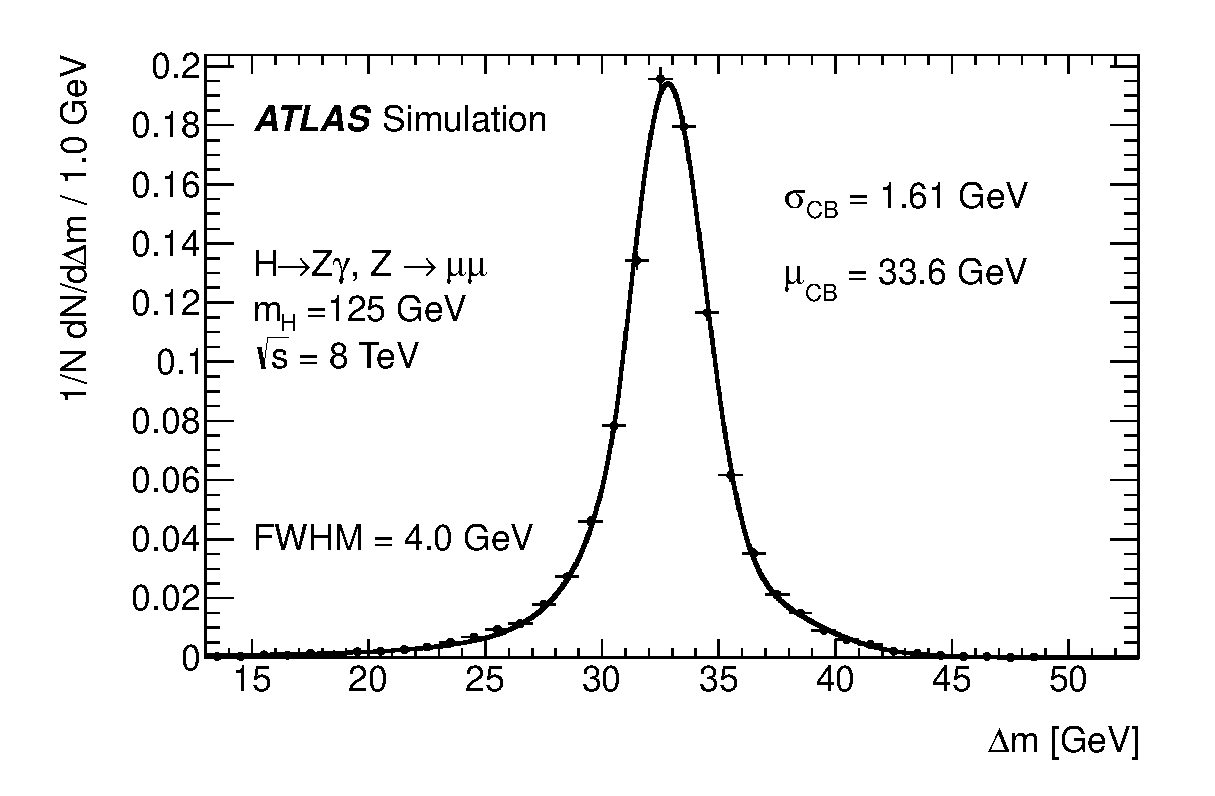
\includegraphics[width=0.46\textwidth]{figures/linPlot_125_EtaZgamma_Cat0_all_mu_mc12a_mDif}}
    \caption{Distribution (normalized to unit area) of the difference $\Delta m$ 
      between the final state three-body invariant mass
      $m_{\ell\ell\gamma}$ and the di-lepton invariant mass
      $m_{\ell\ell}$ for signal events
      passing the full selection (dots), for $m_H = 125$~GeV and $\sqrt{s}=7$ (top) or 8 (bottom) TeV. 
      The line overlaid represents the fit of the distribution with a
      model composed of the sum of a Crystal Ball (CB) and a Gaussian (GA) function.
      Left: electron channel, right: muon channel. 
    }
    \label{fig:resolution_model_example_8tev_H125}
  \end{center}
\end{figure}


\label{sec:signal}

\section{Background Studies}
 \label{sec:background}
In order to distinguish the Higgs boson signal from the background using \dm
as a discriminant, a model for the background distribution is needed. The background
is modeled with a smooth analytic p.d.f. that reproduces the data as well as the 
mixture of background Monte Carlo samples normalized to the data-driven background 
yields. It should be noted that the parameters of the background p.d.f. are not fixed
from simulation, but are fitted on the data. The model was chosen carefully so that
it does not introduce significant biases on the fitted signal while at the same
time preserving the sensitivity to the search.

\subsection{Background model}
A number of functional forms were tested including polynomials of various orders,
as well as non-polynomial functions such as exponential, Crystal Ball+Gaussian,
and Crystal Ball+Landau distributions. The advantage of non-polynomial functions
is that they do not follow the local peaks and troughs of the mass distribution 
that are a result of statistical fluctuations. A high statistics simulated
background-only Monte Carlo sample was used to test the performance of the
signal+background fits of the \dm distribution. This was done by performing
pseudo-experiments\footnote{Data generated by sampling from a known distribution
using a Monte Carlo sampling method. 
The resulting distribution looks like data from the experiment.} 
with a variable amount of Higgs signal events injected in
the mass range 115-135 GeV. For each experiment an unbinned maximum likelihood
fit is performed for a fixed \mllg, and the number of signal events together
with the fitted parameters are obtained. The key result of these tests is
the \emph{spurious signal}, i.e. the bias on the signal. The spurious signal
is defined as the average fitted number of signal events after subtracting
the input signal events ($\average{S} - S_{\text{generated}}$) in units of the
uncertainty in the fitted number of signal events, $\sigma_S$. In order for the
spurious signal to not give a systematic uncertainty on the final result
that is significant compared to the statistical uncertainty of the measurement
itself, we searched for models that yield, for the tested Higgs mass hypotheses,
a spurious signal which is within $\pm20\%$ of the fitted error on the signal yield.

The results for the background-only simulated samples corresponding to 4.6 \ifb
of 2011 data and 20.7 \ifb of 2012 data in the muon and electron channels are
shown in \refF{fig:spurioussignal}. The model that was found to provide the best 
sensitivity to the signal while limiting
the spurious signal to be within $\pm20\%$ of the fitted signal uncertainty, for
both 4.6 \ifb of 2011 data and 20.7 \ifb of 2012, is a third-order 
Chebychev polynomial in the fit range $24 < \dm < 64 \GeV$.

\begin{figure}[htbp]
    \centering
    \begin{subfigure}[b]{0.45\textwidth}
      \centering
      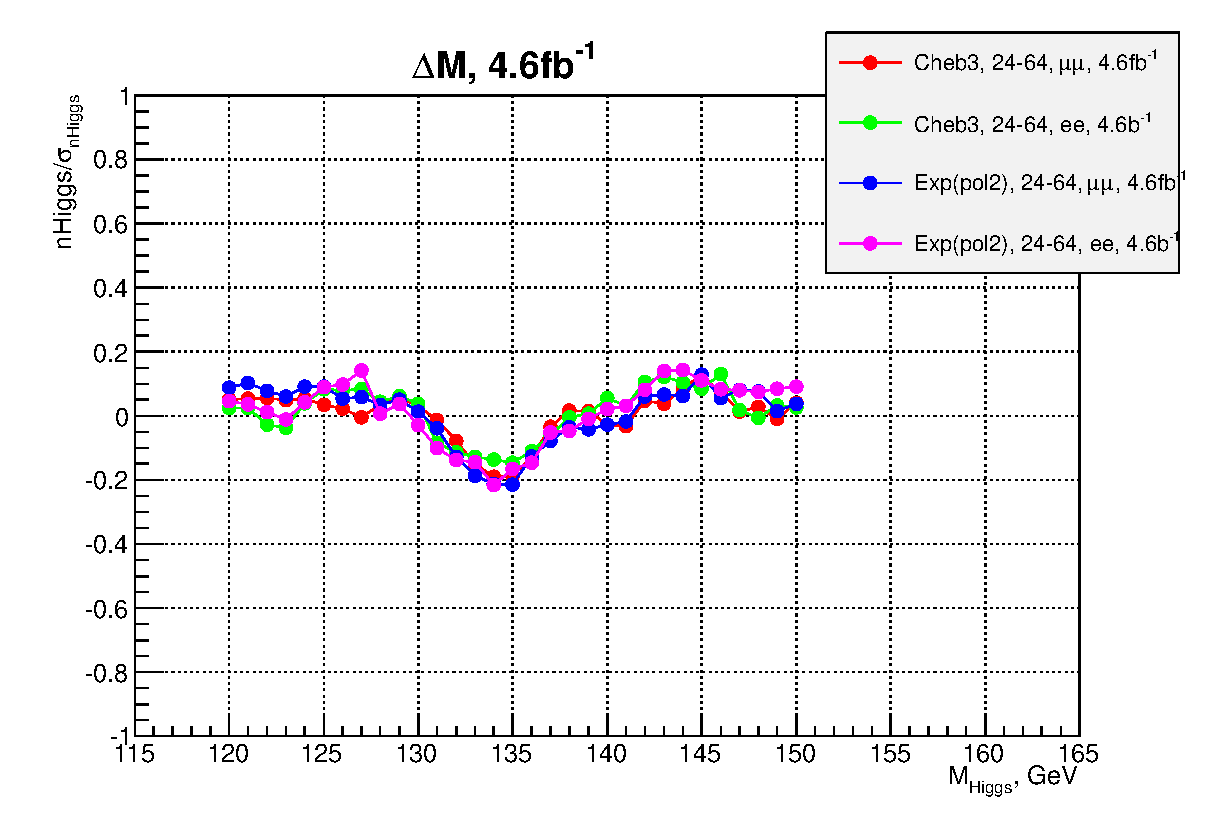
\includegraphics[width=\textwidth]{figures/rat4orig.eps}
      \caption{}
      \label{fig:4spurious}
    \end{subfigure}
    \quad
    \begin{subfigure}[b]{0.45\textwidth}
      \centering
      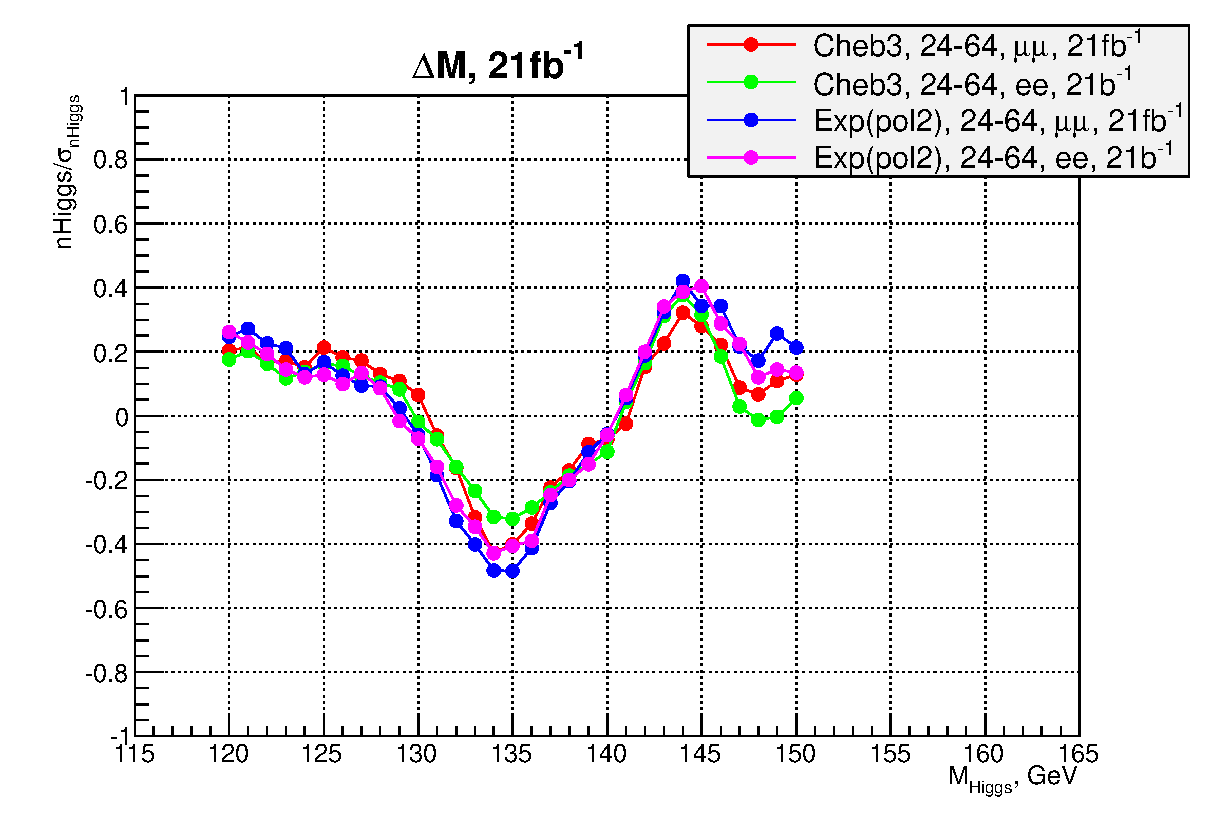
\includegraphics[width=\textwidth]{figures/rat21orig.eps}
      \caption{}
      \label{fig:21spurious}
    \end{subfigure}
    \caption{Number of Higgs candidates divided by uncertainty 
    returned by the fit of the pseudo-data $\Delta M$ distributions averaged over 
    1000 pseudo-experiments with 0 injected Higgs candidates. 
    The statistics corresponds to 4.6 \ifb (Fig.~\ref{fig:4spurious})
    and 21 \ifb (Fig.~\ref{fig:21spurious}). The dip at 135 GeV in the
    $21 \ifb$ sample is due to downward fluctuation in the data at this mass.}
    \label{fig:spurioussignal}
\end{figure}

\subsection{Background-only fits to the data}
The shape parameters and the normalization of the background are determined
by unbinned maximum likelihood fits to the data events selected in the
range $24 \GeV < \dm < 64 \GeV$, performed separately for the two lepton flavors 
and separately for the $\rts = 7 \TeV$ and $\rts = 8 \TeV$ data, using the third-order
Chebychev polynomial selected in the previous section. 
\refF{fig:deltaM_data_bkgonly_fit} shows the background-only fits to the data in the
two categories for the $\rts = 7 \TeV$ and the $\rts = 8 \TeV$ data.

 \begin{figure}[!htbp]
  \begin{center}
    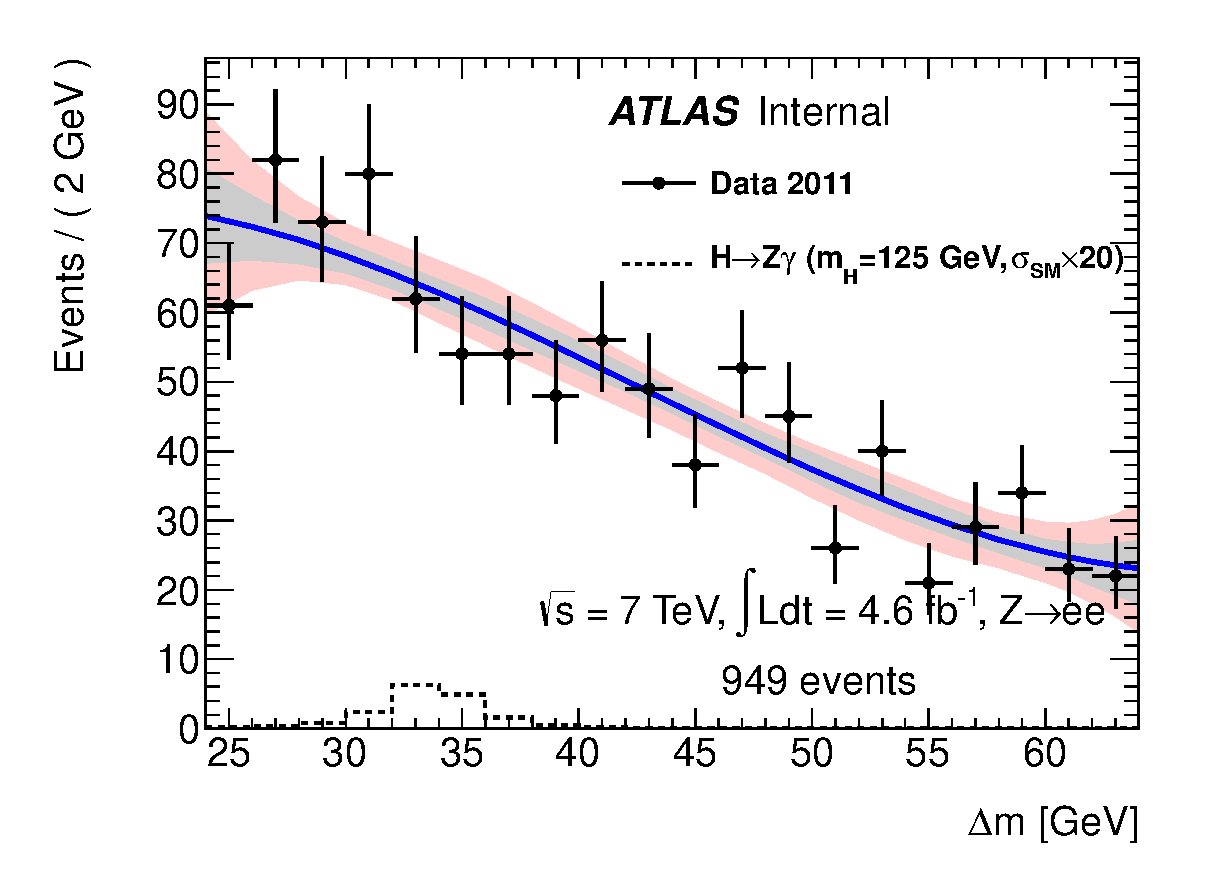
\includegraphics[width=0.49\columnwidth]{figures/bkgplots_e_deltaM_fit_11_CB3_fiterr_internal_withsignal}
    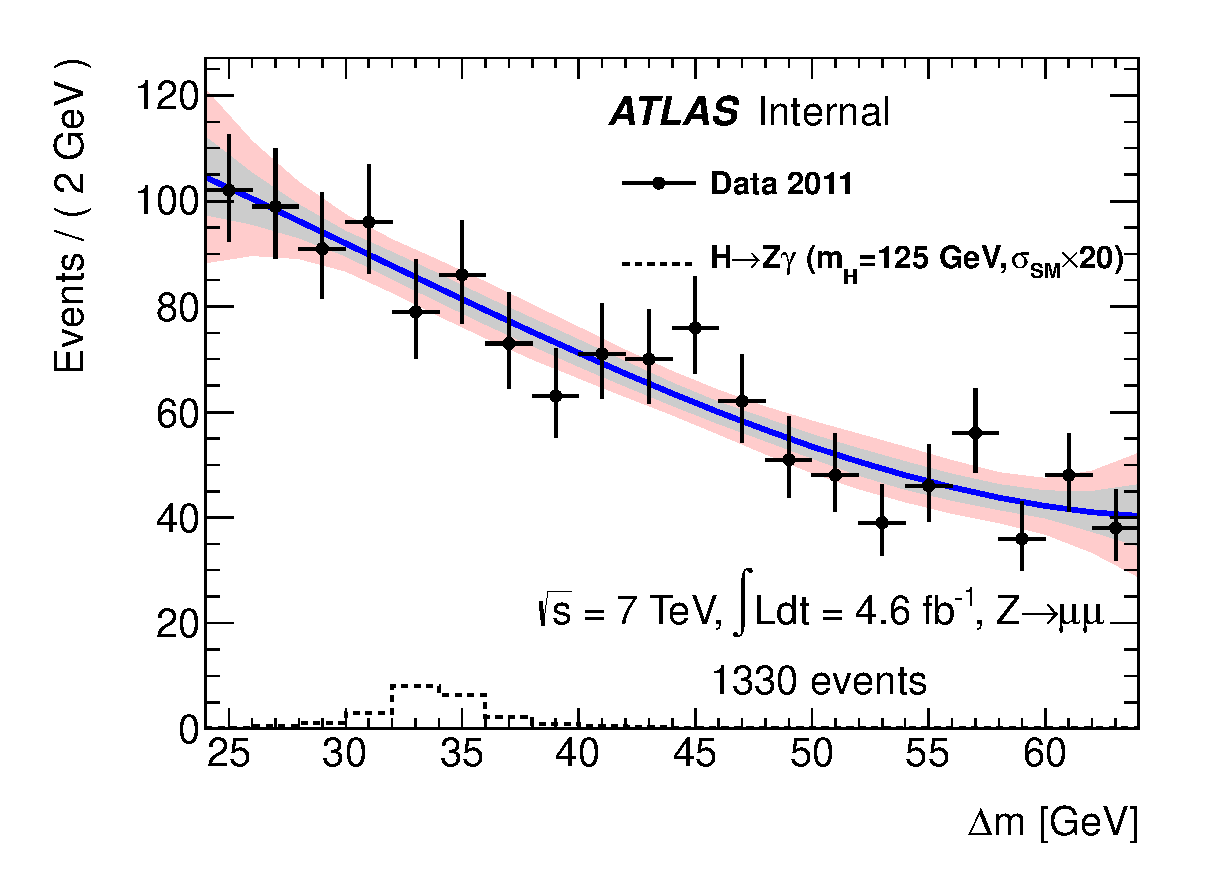
\includegraphics[width=0.49\columnwidth]{figures/bkgplots_mu_deltaM_fit_11_CB3_fiterr_internal_withsignal}
    \includegraphics[width=0.49\columnwidth]{figures/bkgplots_e_deltaM_fit_12_CB3_fiterr_internal_withsignal} 
    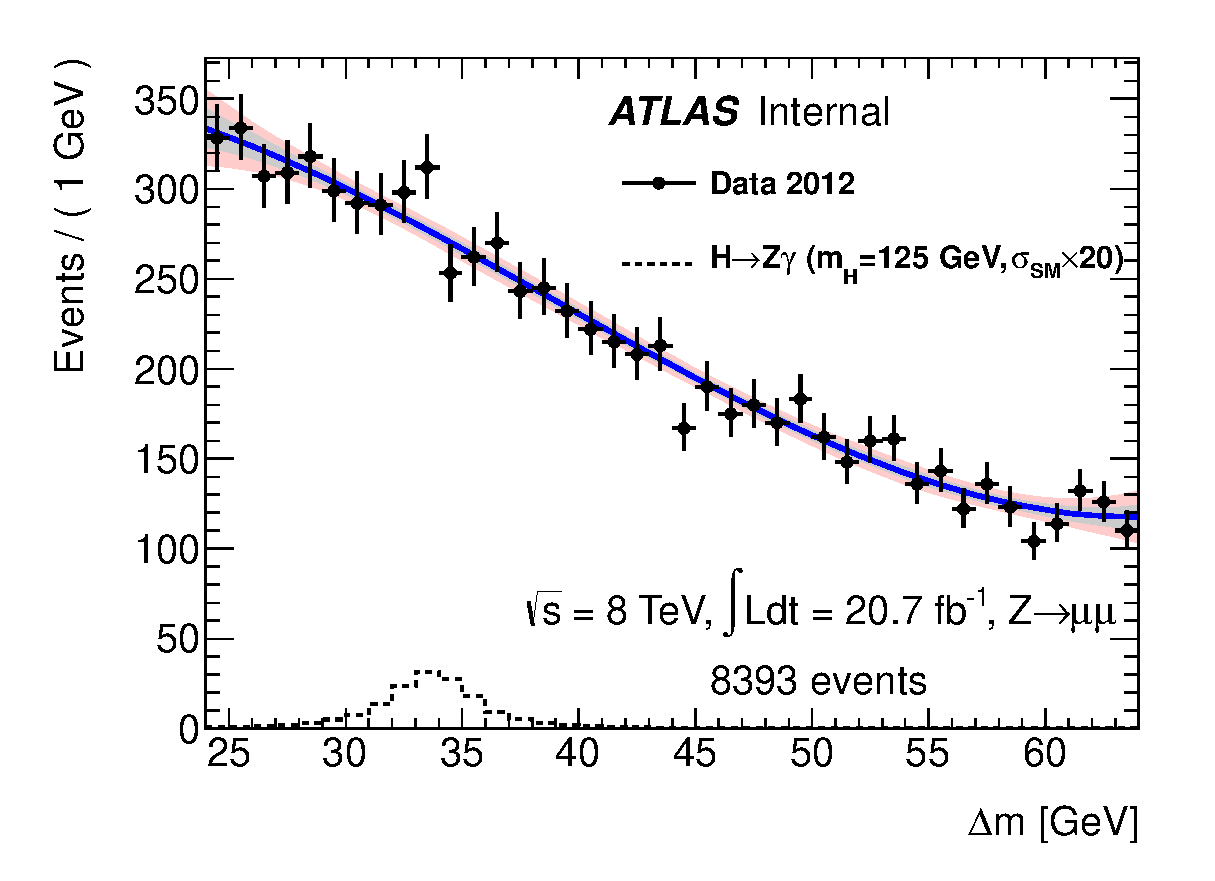
\includegraphics[width=0.49\columnwidth]{figures/bkgplots_mu_deltaM_fit_12_CB3_fiterr_internal_withsignal}
    \caption{Background-only fits to the distribution of 
      the mass difference $\Delta m$ of selected events in data,
      for $Z\to ee$ (left) and $Z\to\mu\mu$ (right), at $\sqrt{s}=7$ 
      TeV (top) or 8 TeV (bottom).
      For both 7 and 8 TeV, a third order polynomial is used for the fit.
      Dots correspond to data, the blue line is the fit result and the gray and light red
      bands are the 1$\sigma$ and 2$\sigma$ uncertainty 
      bands from the statistical uncertainties on the fitted 
      background model parameters.
      The dashed histograms correspond to the SM signal expectation,
      for a Higgs boson mass of 125 GeV, scaled by a factor 20 for clarity.
%%      The pulls of the data points with respect to the fit are also shown.
    }
    \label{fig:deltaM_data_bkgonly_fit}
  \end{center}
\end{figure}

\label{sec:background}

\section{Systematic Uncertainties}
\label{sec:sys}
A complete model of the signal and background distributions not only require
a description of the signal and background shapes observed in data, but also 
a quantification of the various uncertainties involved in the measurement.
The theoretical and experimental systematic uncertainties are summarized in
this section.

\subsection{Theoretical Uncertainties}
There are two sources of theoretical uncertainties on the production cross-section
of \HToZg events: the uncertainty related to the energy scales used for the
fixed-order calculation, and the uncertainty from the parton distribution functions
(PDFs) and the value of $\alphas$ used in the perturbative calculation. 

\begin{itemize}
\item \textbf{Scale Uncertainties:} 
In theoretical calculations, the value of observables are obtained using a 
perturbative expansion. This introduces an uncertainty due to missing higher order
corrections. In particular, the \HToZg signal cross-section is typically calculated
with leading-order (LO) matrix elements that can be corrected with higher-order
QCD (the production of a Higgs boson via gluon fusion is a QCD process) and 
electroweak corrections (Vector Boson Fusion production).

\item \textbf{Proton Structure Uncertainties:}
At the LHC Higgs bosons are produced using proton-proton collisions, so
an understanding of the \HToZg cross-section depends on the internal
parton structure of the proton. This internal proton structure cannot be
extracted from perturbation theory ($\alphas$ is large at the low binding
energies of the proton) and must be measured in the form of parton distribution
functions (PDFs). Consequently, the statistical and systematic uncertainties 
of these measurements must be propagated to any calculated cross-section.
\end{itemize}

The Higgs boson production
cross-sections and decay branching fractions as functions of the Higgs boson
mass are compiled, together with uncertainties, in Ref.~\cite{LHCHiggsCrossSectionWorkingGroup:2011ti}.
For each tested Higgs boson mass hypothesis the uncertainties from Ref.~\cite{LHCHiggsCrossSectionWorkingGroup:2011ti} are used.
\refT{tab:theory_uncertainties} summarizes uncertainties for a Higgs boson mass of
125 GeV. They depend only mildly on $m_H$, for $120 \GeV < m_H < 150 \GeV$,
with the exception of the relative uncertainty on the \HToZg branching fraction,
which varies between 9.4\% at 120 GeV and 6.2\% at 150 GeV.

Theoretical uncertainties on the background cross-sections do not affect the
results shown in the next section, because the background normalization and shape
are obtained through a fit to data.

\begin{table}[!htbp] 
  \renewcommand{\arraystretch}{1.3}
  \begin{center}
    \caption{Theoretical systematic uncertainties for the SM Higgs
      boson production cross section and branching fraction of the
      $H\to Z\gamma$ decay at $\sqrt{s} = 7$ and 8 TeV,
      for a Higgs boson mass of 125 GeV.}
    \label{tab:theory_uncertainties}
%\vspace{1mm}
    \begin{tabular}{l|cc|cc|cc|cc|cc|c}
      \hline\hline
$\sqrt{s}$ & \multicolumn{11}{c}{Systematic uncertainty (\%)}\\
%\hline
           & \multicolumn{2}{c}{$\sigma(gg\to H)$} & \multicolumn{2}{|c}{$\sigma$(VBF)} & \multicolumn{2}{|c}{$\sigma(WH)$} & \multicolumn{2}{|c}{$\sigma(ZH)$} & \multicolumn{2}{|c|}{$\sigma(t\bar tH)$} & $B(H\to Z\gamma)$ \\
         & scale & PDF & scale & PDF & scale & PDF & scale & PDF & scale & PDF & \\
\hline
7 TeV & $^{+7.1}_{-7.8}$  & $^{+7.6}_{-7.1}$  & {\small $\pm 0.3$} & $^{+2.5}_{-2.1}$ & $^{+0.2}_{-0.8}$ & {\small $\pm 3.5$} & $^{+1.4}_{-1.6}$ & {\small $\pm 3.5$} & $^{+3.3}_{-9.3}$  & {\small $\pm 8.5$} & $^{+9.0}_{-8.8}$ \\
8 TeV &$^{+7.3}_{-7.9}$  &$^{+7.5}_{-6.9}$   & {\small $\pm 0.2$} & $^{+2.6}_{-2.8}$ & $^{+0.1}_{-0.6}$ & {\small $\pm 3.4$} & $^{+1.5}_{-1.4}$ & {\small $\pm 3.5$} & $^{+3.9}_{-9.3}$  & {\small $\pm 7.8$} & $^{+9.0}_{-8.8}$ \\
  \hline\hline
    \end{tabular}
  \end{center}
\end{table}

\subsection{Experimental Uncertainties}
The following sources of experimental systematic uncertainties on the expected
signal yields have been considered:
\begin{itemize}
\item \textbf{Luminosity:}
The uncertainty on the integrated luminosity for the 2011 data is 1.8\% 
and $\pm 3.6\%$ in 2012 \cite{ATLAS:2012roa}.
%
\item \textbf{Acceptance of the kinematic requirements:}
The total acceptance of \HToZg events is defined as the ratio of the total number
of \HToZg events that pass all selections divided by the initial number of \HToZg
events. The uncertainties related to the acceptance of the selection criteria are
estimated using Monte Carlo simulations. This yields an uncertainty of 4\%.
%
\item \textbf{Photon identification efficiency:} 
Recall that to have reliable comparison between data and theory one uses Monte Carlo
simulation to generate events by computer randomly following a distribution predicted
by theory. However, there are areas where simulation can not reproduce data exactly
because there is no theory reproducing reality perfectly. In these areas on
need to bring Monte Carlo simulations to the level of data by hand. This is done
with the help of scale factors (SF) which are extracted from variables that are
easy to analyze. One such quantity is the photon identification efficiency scale
factor, which quantifies the discrepancy between data and MC when it comes to
identifying photons in the ATLAS detector. At $\rts = 7 \TeV$, the signal
yield is recomputing by varying the photon identification efficiency scale factors
within their uncertainties and the relative variation is considered as a systematic
uncertainty. At $\rts = 8 \TeV$ a conservative estimate of the uncertainty on the
photon identification efficiency obtained from a comparison between data-driven
measurements and the simulated efficiencies is used. This amounts to 2.5\% for
$\et < 40 \GeV$ and for unconverted photons with $\abseta > 1.81$ and to 1.5\%
otherwise. The resulting uncertainty on the \HToZg selection efficiency is below
3\%.
%
\item \textbf{Photon and electron calorimeter isolation requirements:}
The signal efficiency defined as $N_{\text{selected}}/N_{\text{truth}}$ 
is measured from simulated events. 
To estimate the systematic uncertainty due to the uncertainty
on the efficiency of the isolation criteria, the signal efficiency is recomputed
by shifting, in the simulation, the photon and electron calorimeter isolation
energies by the average difference observed between data and Monte Carlo for
photons and electrons, selected either in di-photon enriched events or
in a control sample of electrons from $Z \to ee$. These difference are of the
order of 100 MeV for the topological-cluster based isolation. The systematic
uncertainty on the signal efficiency range between 0.2\% and 0.4\%.
%
\item \textbf{Photon and electron energy scales:}
The energy of electromagnetic particles is measured by the electromagnetic 
calorimeter essentially through a measurement of the amount light produced by
the particle's interactions with the calorimeter's material. However, there
are a number of effects that spoil the accuracy of the conversion of light into
a particle's energy. The particles may punch through the calorimeter without leaving
their energy inside, or they hit parts of the device which are uninstrumented or
malfunctioning. Therefore, a correction to the energy measured in the 
electromagnetic calorimeter is applied known as an energy scale factor, which
rescales the measured energy to match the one the original particle had.

The uncertainty from the electromagnetic (photon and electron) energy
scales is assessed by varying the electromagnetic scale corrections (applied
to the data) within their uncertainties. The effects of the uncertainty fomr
the $Z \to ee$ calibration sample used to to extract the scale factors, of the
limited knowledge of the material, of the uncertainty on the pre-sampler energy 
scale and the low-$\pt$ scale factor uncertainties are evaluated. The total
uncertainty on the signal efficiency is around 0.2\% for events in which
the $Z$ boson candidate decays to muons and between 0.4\% and 1.2\% for
events in which the $Z$ boson candidate decays to electrons.
%
\item \textbf{Photon and electron energy resolution:}
The measurement of the electromagnetic energy only has a finite resolution.
The uncertainty from this electromagnetic energy resolution is estimated by
varying the resolution smearing corrections within its uncertainties and
observing the relative variation in the predicted signal yield. The estimated
uncertainty is smaller than 0.2\%.
%
\item \textbf{Electron trigger, reconstruction, and identification efficiency:}
The electron trigger, reconstruction, and identification efficiency uncertainties
are estimated by varying the efficiency scale factors applied to the simulation within
their uncertainties. The total uncertainty, for events in which the $Z$ boson
candidate decays to electrons, is around 3\%.
%
\item \textbf{Muon momentum scale and resolution:} 
The uncertainty of the efficiency of the $\pt > 10 \GeV$ cut (15 GeV for muons
tagged in the calorimeters) is estimated by varying the muon momentum
corrections in MC by their uncertainties. The effect is around 0.1\%.
%
\item \textbf{Muon trigger, reconstruction, and identification efficiency:}
The trigger, reconstruction, and identification muon efficiency uncertainties
are estimated by varying the efficiency scale factors within their uncertainties.
The total uncertainty, for events which $Z$ boson candidate decays to muons, is
below 1\%.
\end{itemize}
Other sources of uncertainties have been estimated by comparing the efficiencies
in data and Monte Carlo for control samples of leptons from $Z$ decays and found to
be negligible. The total relative uncertainty in the signal efficiency is around 5\%.

The following sources of experimental systematic uncertainties on the signal \dm
distribution have been considered:
\begin{itemize}
\item \textbf{Photon and energy scales:}
The signal \dm distribution is recomputed after varying the electromagnetic
energy scale corrections within their uncertainties, and the shift of the
peak position (0.2 GeV) is considered the systematic uncertainty.
%
\item \textbf{Photon and electron energy resolution:}
The signal \dm distribution is recomputed after varying the electromagnetic
smearing corrections within their uncertainties, and the relative variation of
its width is taken as a systematic uncertainty. It amounts to 2-4\% for events
in which the $Z$ boson candidate decays to muons and to 5\% for events in which the 
$Z$ boson candidate decays to electrons.
%
\item \textbf{Muon momentum scale:}
The signal \dm distribution is recomputed after varying the muon momentum scale
within its uncertainties, and the shift of the peak position is considered
as a systematic uncertainty. This uncertainty is found to be negligible.
%
\item \textbf{Muon momentum resolution:}
The signal \dm distribution is recomputed after varying the muon momentum smearing
corrections within their uncertainties, and the relative variation of its
width (0-1.5\%) is taken as a systematic uncertainty.
\end{itemize}

The list of the main sources of systematic uncertainties and their contributions
to the \HToZg expected signal yields and parameters of the signal \dm distributions
are listed in Table~\ref{tab:zg_syst_125_8_7tev} for $m_H = 125 \GeV$ and
$\rts = 8$ (7) TeV. The systematic uncertainties are profiled in the final
maximum likelihood fit to the data, as described in \refS{subsec:nuisance}. All
systematic uncertainties, except that on the luminosity, are treated as
correlated between $\rts = 7 \TeV$ and the $\rts = 8 \TeV$ analyses.

\begin{table}[!htbp]
\centering
\caption{Summary of the systematic uncertainties on the signal yield and
  invariant mass distribution for $m_H = 125$ GeV, at $\sqrt{s}=8 (7)$ TeV.}
  \label{tab:zg_syst_125_8_7tev} 
\small
 \begin{tabular}{cccc}
       \hline
       \hline
       \textbf{Systematic Uncertainty }           & $H \rightarrow Z(ee) \gamma$(\%)   & $H \rightarrow Z(\mu\mu) \gamma$(\%) \\
       \hline
       \textbf{Signal Yield}                      &                                    &                                      \\ 
       \hline
       \multicolumn{1}{l}{Luminosity}                                 & 3.6 (1.8)                        & 3.6 (1.8)          \\
       \multicolumn{1}{l}{Trigger efficiency}                         & 0.4 (0.2)                        & 0.8 (0.7)          \\
       \multicolumn{1}{l}{Acceptance of kinematic selection}          & 4.0 (4.0)                        & 4.0 (4.0)          \\
       \multicolumn{1}{l}{$\gamma$ identification efficiency}         & 2.9 (2.9)                        & 2.9 (2.9)          \\  
       \multicolumn{1}{l}{electron reconstruction and identification efficiency} & 2.7 (3.0)             &                    \\  
       \multicolumn{1}{l}{$\mu$ reconstruction and identification efficiency}    &                       & 0.6 (0.7)          \\  
       \multicolumn{1}{l}{$e/\gamma$ energy scale}                    & 1.4 (0.3)                        & 0.3 (0.2)          \\
%%       \multicolumn{1}{r}{Method uncertainty ($Z\to ee$)} & \multicolumn{1}{r}{1.4 (0.2)}   & \multicolumn{1}{r}{0.2 (0.1)} \\
%%       \multicolumn{1}{r}{Material uncertainty}   & \multicolumn{1}{r}{0.1 (0.1)}    & \multicolumn{1}{r}{0.2 (0.1)}        \\
%%       \multicolumn{1}{r}{Presampler energy scale}& \multicolumn{1}{r}{0.0 (0.1)}    & \multicolumn{1}{r}{0.0 (0.0)}        \\
%%       \multicolumn{1}{r}{Low pt}                 & \multicolumn{1}{r}{0.2 (0.2)}    & \multicolumn{1}{r}{0.2 (0.1)}        \\
       \multicolumn{1}{l}{$e/\gamma$ isolation}                       & 0.4 (0.3)                        & 0.4 (0.2)          \\  
       \multicolumn{1}{l}{$e/\gamma$ energy resolution}               & 0.2 (0.2)                        & 0.0 (0.0)          \\
       \multicolumn{1}{l}{$\mu$ momentum scale}                       &                                  & 0.1 (0.1)          \\  
       \multicolumn{1}{l}{$\mu$ momentum resolution}                  &                                  & 0.0 (0.1)          \\
       \hline
       \textbf{Signal $\Delta m$ resolution}      &                                    &                                      \\  
       \hline 
       \multicolumn{1}{l}{$e/\gamma$ energy resolution}               & 5.0 (5.0)                        & 2.4 (2.4)          \\ 
       \multicolumn{1}{l}{$\mu$ momentum resolution}                  &                                  & 0.0 (1.5)          \\
       \hline
       \textbf{Signal $\Delta m$ peak position} \\
       \hline
       \multicolumn{1}{l}{$e/\gamma$ energy scale}                    & 0.2 (0.2) GeV                    & 0.2 (0.2) GeV    \\
       \multicolumn{1}{l}{$\mu$ momentum scale}                       &                                  & negligible         \\
       \hline
       \hline
 \end{tabular}
\end{table}

\label{sec:sys}

\section{Results}
\label{sec:results}

\subsection{Statistical method for the evaluation of limits and $p$-values}
\label{subsec:statintro}
Evidence for \HToZg production at the LHC would be an excess of Higgs bosons 
in the \dm or \mllg invariant mass distributions over the background of known
Standard Model processes. As such, likelihood-based statistical tests are used to
interpreted the selected data samples in terms of the SM background plus the 
contribution of a Standard Model Higgs boson decaying to $Z\gamma$.
The results are expressed in terms of a ``signal-strength" parameter 
$\mu$, which is defined as the ratio
\[
    \mu = \frac{N_{\text{signal}}}{N_{\text{signal}}^{\text{SM}}}
\]
of the measured number of signal events to the value expected by the
Standard Model. For a Standard Model Higgs boson decaying to $Z\gamma$,
the value of $\mu$ should be consistent with unity within statistical uncertainties.

First, in order to quantify the significance of a possible observation,
a hypothesis test is performed to evaluate the
compatibility between the data and the null hypothesis, which assumes
that the selected data contains only background events. If the hypothesis
test shows no presence of any significant excess in the data, 
a limit on the ratio of the \HToZg cross-section over the Standard Model 
expectation is set. These results are quoted for a possible Higgs boson mass 
between 120 and 150 GeV.

\subsubsection{$p$-value calculation}
Any statistical hypothesis test begins by defining two competing hypothesis:
the null and alternate hypothesis. Here the null hypothesis corresponds to the
hypothesis that the data contains only Standard Model background processes 
($\mu = 0$), i.e. the background-only (B-only) hypothesis. 
In contrast, the alternate hypothesis is the conjecture that a Standard Model
Higgs boson is contained in the data ($\mu = 1$). This hypothesis is also known
as the signal plus background (S+B) hypothesis. The compatibility of the
data with the background-only hypothesis is quantified by the $p_0$ or $p$-value
of the data, which gives the probability for a dataset generated in the
B-only hypothesis to be in the same or worse agreement with that hypothesis.
Only upward deviations from the B-only hypothesis, which would correspond to
a positive signal strength, are considered. Large \pzero therefore correspond
to datasets that agree well with the B-only hypothesis, while small \pzero can
be interpreted as a suggestion of a significant positive signal.

In order to investigate the measure of agreement between the observed data
and a given hypothesis, one constructs a function of the data
called a test statistic. The test statistic is designed to reduce a large
quantity of data points to a single value whose distribution can be used to
distinguish the null from the alternative hypothesis through a 
hypothesis test. Following the ATLAS recommendations~\cite{ATLAS_stat_recommendations}
, the \pzero is computed from the $q_0$ test statistic, defined as
\[
    q_0 =
    \begin{cases}
        -2\ln{\frac{L(0,\hat{\hat\theta}(0))}{L(\hat\mu,\hat\theta)}} & \hat\mu \ge 0 \\
        +2\ln{\frac{L(0,\hat{\hat\theta}(0))}{L(\hat\mu,\hat\theta)}} & \hat\mu < 0
    \end{cases}
\]
where $L$ is the likelihood function described in \refS{subsec:likelihood},
$\hat \mu$ and $\hat \theta$ are the best-fit values for $\mu$ and $\theta$
with all parameters floating, and $\hat{\hat\theta}(0)$ is the best-fit value of
$\theta$ in the B-only ($\mu=0$) hypothesis. 

In the expression for $\hat\mu > 0$, 
the numerator corresponds to the best value of the likelihood computed in the
B-only hypothesis, while the denominator corresponds to the best value in the
S+B hypothesis including both signal and background. Therefore, for datasets 
compatible with the B-only hypothesis, both should be of similar magnitude and
$q_0$ will be small. Conversely, in the presence of a signal the denominator
(S+B hypothesis) should be much larger than the numerator (B-only hypothesis),
yielding a large value for $q_0$. These observations lead to the following
definition for the $p$-value of the null hypothesis:
\[
    p_0 = \int_{q_{0,\text{obs.}}}^{\infty} f(q_0|0,m_H,\hat{\hat\theta}(0))\,dq_0
\]
where $f$ is the distribution of the test statistic. An illustration of this 
calculation is presented in \refF{fig:pvalue}. This definition is equivalent
to saying that the $p$-value gives the probability for a dataset generated in the
null hypothesis to be in the same or worse agreement with that hypothesis since
large values of $q_0$ correspond to the data being incompatible with the B-only
hypothesis. In this scheme, small $p_0$ occurs only for $q_0 > 0$, which happens
only for $\hat\mu \ge 0$. This corresponds to the one-sided prescription mentioned
above, where only positive (``physical") values of the signal are considered. 
Negative fluctuations of the  signal are assigned $p_0$ values in the interval
$[0.5,1]$, with values close to 0.5 corresponding to small negative fluctuations,
and values close to 1 for large negative fluctuations.

\begin{figure}[htbp]
    \centering
    \includegraphics[scale=0.4, angle=0]{./figures/pvalue}
    \caption{Illustration of the relation between the $p$-value obtained from an
    observed value of the test statistic $t_{\mu}$ (this corresponds to $q_0$ in
    the discussion presented in this paper). This figure is taken from 
    \cite{Cowan:2010js}.}
    \label{fig:pvalue}
\end{figure}

It should be noted that in the asymptotic regime, which is usually a good
approximation for the models studied here, $p_0$ values can be directly computed
from the $q_0$ values using a closed form asymptotic formulae \cite{Cowan:2010js}.
Alternatively, the \pzero can be computed by sampling the distribution of $q_0$
in the B-only hypothesis using pseudo-experiments. Unless otherwise stated, 
asymptotic formulae will be used in the results presented here. In the following,
we present both \emph{observed} $p_0$ results, computed using real data, and
\emph{expected} $p_0$, which are computed from an Asimov dataset\footnote{
An Asimov dataset is defined such that when one uses it to evaluate the 
estimators for all parameters, one obtains the true parameter values.}
in the $\mu = 1$ hypothesis.

\subsubsection{Limit-setting}
If one finds that the data is compatible with the B-only hypothesis, then this
is an indication that there is not a significant excess of signal in the data
(it does not rule out the S+B hypothesis). The question that is then asked is
how large the signal's production cross-section can be before one would expect
to measure signal events with the amount of data collected so far. 
If the upper limit on the signal strength $\mu$ lies
below unity indicating that less Higg's bosons are produced then predicted by 
the Standard Model, then that is an indication that the S+B hypothesis is incorrect.

Upper limits on the signal strength are set using a modified frequentest ($CL_s$)
method \cite{cls}, using a $CL_{s+B}$ based on the \qmu test statistic,
as recommended by the ATLAS Collaboration \cite{ATLAS_stat_recommendations}. 
The test statistic is computed as
\[
    \tilde q_{\mu} =
    \begin{cases}
        -2\ln{\frac{L(\mu,\hat{\hat\theta}(\mu))}{L(\hat\mu,\hat\theta)}} & 0 \le \hat\mu \le \mu \\
        0 & \hat\mu > \mu \\
        -2\ln{\frac{L(0,\hat{\hat\theta}(0))}{L(\hat\mu,\hat\theta)}} & \hat\mu < 0
    \end{cases}
\]
where $L$ is the likelihood function described in \refS{subsec:likelihood},
$\hat\mu$ and $\hat\theta$ are the best-fit values for $\mu$ and $\theta$ with
all parameters floating, and $\hat{\hat\theta}(\mu)$ is the best-fit value for
$\theta$ for a fixed value of $\mu$. The statistic estimates the compatibility 
of the data with the $\mu$ hypothesis using the ratio of likelihoods for the case
of floating $\mu$ (denominator), and the case where it is fixed at the hypothesis
value (numerator). As for the case of $q_0$, a one-sided prescription is used,
assigning $\qmu = 0$ if the fitted value $\hat\mu$ is above the hypothesis.
Finally, if $\hat\mu < 0$, the case $\mu=0$ is used instead to avoid technical
issues with negative p.d.fs.

The $CL_{s+b}$ $p$-value is defined as:
\[
    p_{s+b} = \int_{\tilde q_{\mu,\text{obs.}}}^{\infty} f(\qmu|\mu,m_H,\hat{\hat\theta}(\mu))\,d\qmu
\]
and the $CL_s$ $p$-value is
\[
    p_{\mu} = \frac{p_{s+b}}{p_b}
\]
where
\[
    p_{b} = 1 - \int_{\tilde q_{\mu,\text{obs.}}}^{\infty} f(\qmu|0,m_H,\hat{\hat\theta}(0))\,d\qmu.
\]
is the $CL_b$ $p$-value. A description of the various $p$-values used in the $CL_s$
exclusion method is presented in \refF{fig:cls}.
The value of $p_{\mu}$ and of the corresponding $CL_s$ exclusion are obtained
using either asymptotic formulae \cite{Cowan:2010js} or pseudo-data generation.
Limits at a 95\% confidence level on the value of the signal strength $\mu$ are
then computed by scanning values of the $\mu$ hypothesis, computing the $CL_s$
exclusions and identifying $\mu_{\text{up}}$ for which this value equals 0.05.

\begin{figure}[htbp]
    \centering
    \includegraphics[scale=0.4, angle=0]{./figures/CLs}
    \caption{The distribution of the statistic $q = -2\ln(L_{s+b}/L_b)$ under the 
    hypotheses $\mu=0$ and $\mu=1$. The $CL_s$ exclusion is defined as the ratio
    between $p_{s+b}$ and $p_{b}$. This figure was taken from \cite{Cowan:2010js}.}
    \label{fig:cls}
\end{figure}

We will present both observed limits, computed using real data, and expected limits
computed using an Asimov dataset generated in the $\mu=0$ hypothesis.

\subsection{Likelihood}
\label{subsec:likelihood}
When performing a hypothesis test on a set of data, one needs a function that 
quantifies the probability of those observations given a set of parameters
set by the hypothesis. In particle physics experiments at ATLAS, a discovery
of a new particle typically proceeds through an analysis of 
invariant mass distributions, such as \dm or \mllg, whose shape and normalization 
are determined by the B-only and S+B hypotheses. 
Given an observed invariant mass distribution one wants
to quantify the probability of observing this distribution given the predictions of 
the Standard Model. The answer to this question is obtained using an 
unbinned maximum likelihood (ML) depending on a single observable $x$, which
is either the invariant mass \mllg or the invariant mass difference \dm. As
mentioned in \refS{subsec:statintro}, we consider a single parameter of interest
in the model, the signal strength $\mu$. In addition to $\mu$, the likelihood
depends on several additional \emph{nuisance} parameters, like the number of
background events or the parameters characterizing the probability distribution
functions of the variable $x$ for signal and background events. For some of
these nuisance parameters, additional prior information may be available, for 
instance from theoretical calculations or from measurements performed in control
samples; in that case, the corresponding probability density function for those
parameters is incorporated into the full likelihood function as described in
\refS{subsec:nuisance}.

The data is split into four discrete, orthogonal categories: two categories,
depending on the flavor of leptons produced by the $Z$ decays ($\ell = e, \mu$),
for each of the two center-or-mass energies (7 and 8 TeV) at which the data was
collected. In order to extract the results, a simultaneous unbinned maximum
likelihood fit to the distribution of $c$ in all the categories was performed.
The full likelihood is written as:
\[
    L\left(\mu,\theta=\bigcup_{c=1}^{n_{cat}}\theta_c|x=\bigcup_{c=1}^{n_{cat}} 
    x_c\right) = 
    \prod_{c=1}^{n_{cat}} L_c(\mu,\theta_c|x_c)
\]
where $n_{cat}=4$ is the number of categories, $\theta_c$ are the nuisance
parameters used to describe the model in category $c$ and $x_c$ is the set of
experimental measurements of the observable $x$ in the same category. $L_c$
is the likelihood in category $c$:
\[
    L_c(\mu,\theta_c|x_c) = \frac{({N'}_c)^{N_c} e^{-{N'}_c}}{N_c !} \prod_{k=1}^{N_c}
    \mathcal{L}_c(x_k|\mu,\theta_c) = 
    \text{Pois}(N_c|{N'}_c) \prod_{k=1}^{N_c} \mathcal{L}_c(x_k|\mu,\theta_c) 
\]
where $N_c$ is the number of selected events, $x_k$ is the value of $x$ measured
in event $k$, $N_{\text{signal},c}$ and $N_{\text{bkg},c}$ are the number of
signal and background events, and ${N'}_c = (N_{\text{signal},c} + N_{\text{bkg},c})$
where each quantity refers to category $c$. The term outside the product is a
Poisson probability factor for ${N'}_c$, which when maximizing the likelihood with
respect to ${N'}_c$ will force the maximum likelihood (ML) estimates of the signal
and background yields to satisfy $\hat N_{\text{signal},c} + \hat N_{\text{bkg},c} =
N_c$. $\mathcal{L}_c(x_k|\mu,\theta_c)$ is the per-event likelihood, i.e. the 
probability, for category $C$, to measure the value $x=x_k$ if the values
of the strength parameter and the nuisance parameters are $\mu$ and $\theta_c$.
Except where otherwise stated, it is taken to be of the form
\[
    \mathcal{L}_c(x|\mu,\theta_c) = \frac{N_{\text{signal},c}(\mu,\theta_c^{\text{norm}})}{N_{\text{signal},c} + N_{\text{bkg},c}}\, f_{\text{signal},c}(x|\theta_c^{\text{shape}}) 
    + \frac{N_{\text{bkg},c}}{N_{\text{signal},c} + N_{\text{bkg},c}}\, f_{\text{bkg},c}(x|\theta_c^{\text{bkg}})
\]
where $f_{\text{signal},c}$ and $f_{\text{bkg},c}$ are the signal and background
probability distribution functions for category $c$, and $\theta_c^{\text{norm}}$,
$\theta_c^{\text{shape}}$, and $\theta_c^{\text{bkg}}$ are the nuisance parameters
used in the description of the expected signal yield, the signal p.d.f., and the
background p.d.f. respectively. The full set of nuisance parameters for each category
$c$ can thus be identified as 
$\theta_c = \theta_c^{\text{norm}} \cup \theta_c^{\text{shape}} \cup 
\theta_c^{\text{bkg}} \cup N_{\text{bkg},c}$. The treatment of systematic 
uncertainties on this physics model are described in \refS{subsec:nuisance}.


\subsection{Treatment of systematic uncertainties}
\label{subsec:nuisance}
In order to incorporate systematic uncertainties into the calculation
of $p$-values and confidence intervals described in the previous section,
an assignment of p.d.f.s to relative uncertainties in the measurement
must be carried out.
In particular, a nuisance parameter $\theta$ is associated with each source
of uncertainty, so that that the signal yields or parameters of the model
becomes functions of $\theta$. One then incorporates a ``penalty" or ``constraint"
term into the final calculation, which exploits the best estimate that we have
of each systematic uncertainty. The nuisance parameters are then fitted (``profiled")
to the data, together with the parameters of interest, when minimizing $-\log L$.
 
In practice, the systematic uncertainties follow either a Gaussian or Log-normal 
form, which depends on the source of the uncertainty. 
If the systematic uncertainty affects the expected signal yield,
the Log-normal form is used to avoid the negative tails. While if it represents
a migration between categories (lepton flavor in the final state), the Gaussian
form is used. For a systematic uncertainty $\sigma$ for which a Gaussian constraint 
is assumed, a nuisance parameter $\theta$ is added that samples from a normal 
distribution $G$ and the constraint term is of the form
\[
    (1 + \sigma\theta),
\]
i.e. the product $A_0 \, G(\theta)\,(1+\sigma\theta)$ is a p.d.f for an observable 
$A$ with mean equal to some nominal value $A_0$ and width equal to the systematic
uncertainty $\sigma$. Similarly, for a systematic uncertainty $\sigma$ for which
a Log-normal constraint is assumed, a nuisance parameter $\theta$ is added
that samples from a normal distribution and the constraint term is of the form
\[
    e^{\sqrt{\log(1+\sigma^2)}\theta}
\]
i.e. the logarithm of the quantity $\exp({\sqrt{\log(1+\sigma^2)}\theta)}$ has
a Gaussian p.d.f. with mean 0 and width equal to one. In the cases where the
uncertainty is asymmetric, a bifurcated Gaussian is actually used as a
constraint instead of a Gaussian. In this case the $\sigma$ is taken to be the
negative uncertainty, and the ratio of positive to negative uncertainties is used
as the right width of the bifurcated Gaussian. The left width is taken to be unity.
As in other ATLAS Higgs searches, all systematic uncertainties except the 
luminosity ones are considered fully correlated between 2011 and 2012 datasets.
 
\subsection{Comparison to the background-only hypothesis and exclusion limits} 
The expected and observed \pzero values are shown in \refF{fig:ExpectedP0_1}
as a function of the Higgs boson mass. Using the full 2011 and 2012 ATLAS data,
corresponding to 4.6 \ifb of $pp$ collisions at $\rts = 7 \TeV$ and 20.7 \ifb
of $pp$ collisions at $\rts=8\TeV$, the expected \pzero ranges between 0.40
and 0.46 for $120 < m_H < 150 \GeV$, corresponding to a significance of 0.25$\sigma$.
The observed \pzero distribution is compatible with the data being composed of
background only. The smallest \pzero (0.042) corresponds to a significance of
$1.61\sigma$, occurs for a mass of 141 GeV. The expected \pzero at $m_H = 125 \GeV$
is 0.443, corresponding to a significance of $0.14\sigma$, while the observed one
is 0.188 (0.89$\sigma$).

\begin{figure}[!htbp]
\centering
    {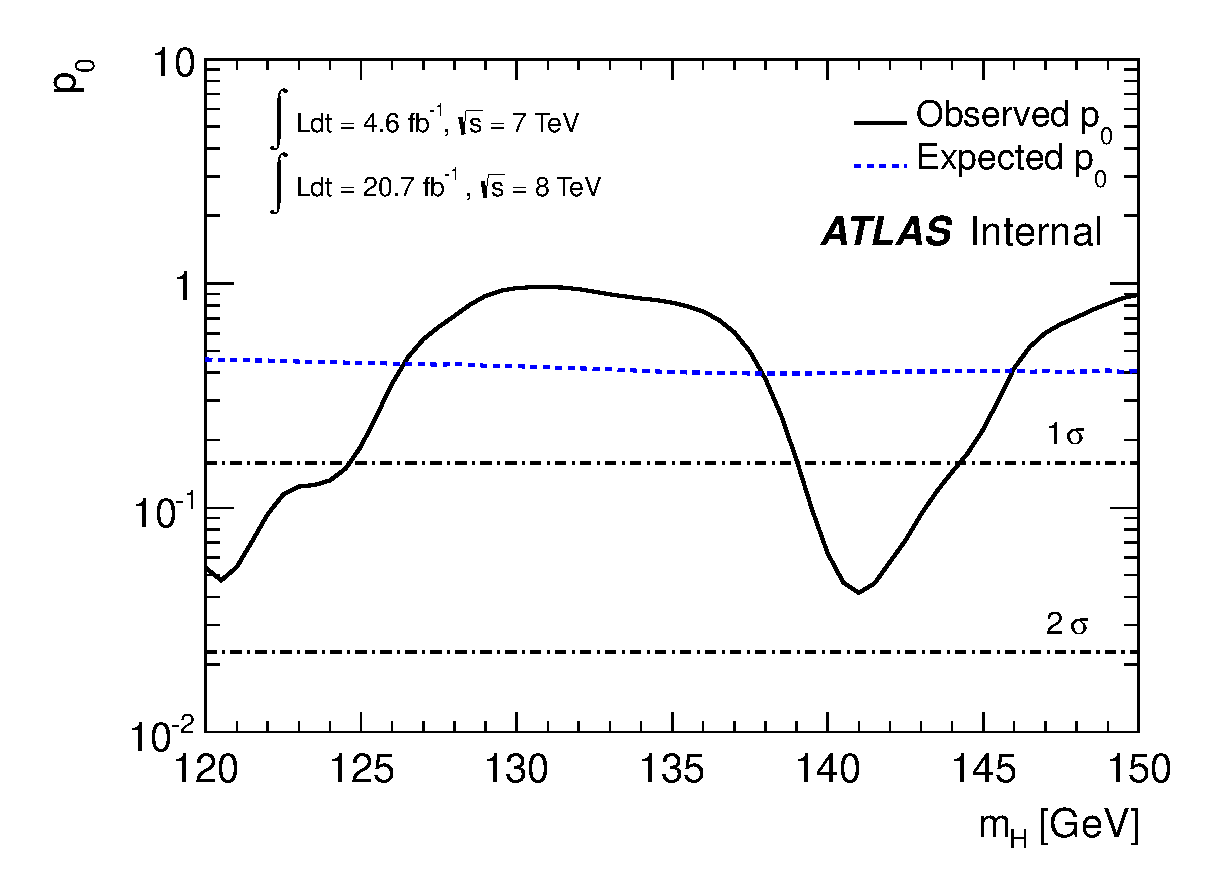
\includegraphics[totalheight=9cm,angle=0]{figures/plot_p0}}
    \caption{Expected (dashed blue line) and observed 
      (solid black line) $p_0$ (compatibility of
      the data with the background-only hypothesis) as a function
      of the Higgs boson mass, using \lumiseventev~\ifb\ of $pp$
      collisions at $\sqrt{s}=7$~TeV and \lumieighttev~\ifb\ of $pp$
      collisions at $\sqrt{s}=8$~TeV.}
    \label{fig:ExpectedP0_1}
\end{figure}

Subsequently, upper limits on the production cross-section of \HToZg are set.
Both observed limits, computed using real data, and expected limits, computed
Asimov dataset generated with the $\mu=0$ hypothesis are shown in 
\refF{fig:ExpectedExclusion_1}. The expected 95\% $CL_s$ limit ranges between
7.3 and 22 and the observed one varies between 5.4 and 37 for a Higgs boson
mass between 120 and 150 GeV. In particular, for a mass of 125 GeV, consistent
with the mass of the recently discovered Higgs-like boson, the expect and observed
limits are equal to 13.5 and 18.2 times the Standard Model, respectively. The
results are dominated by the statistical uncertainties.

\begin{figure}[!htbp]
\centering
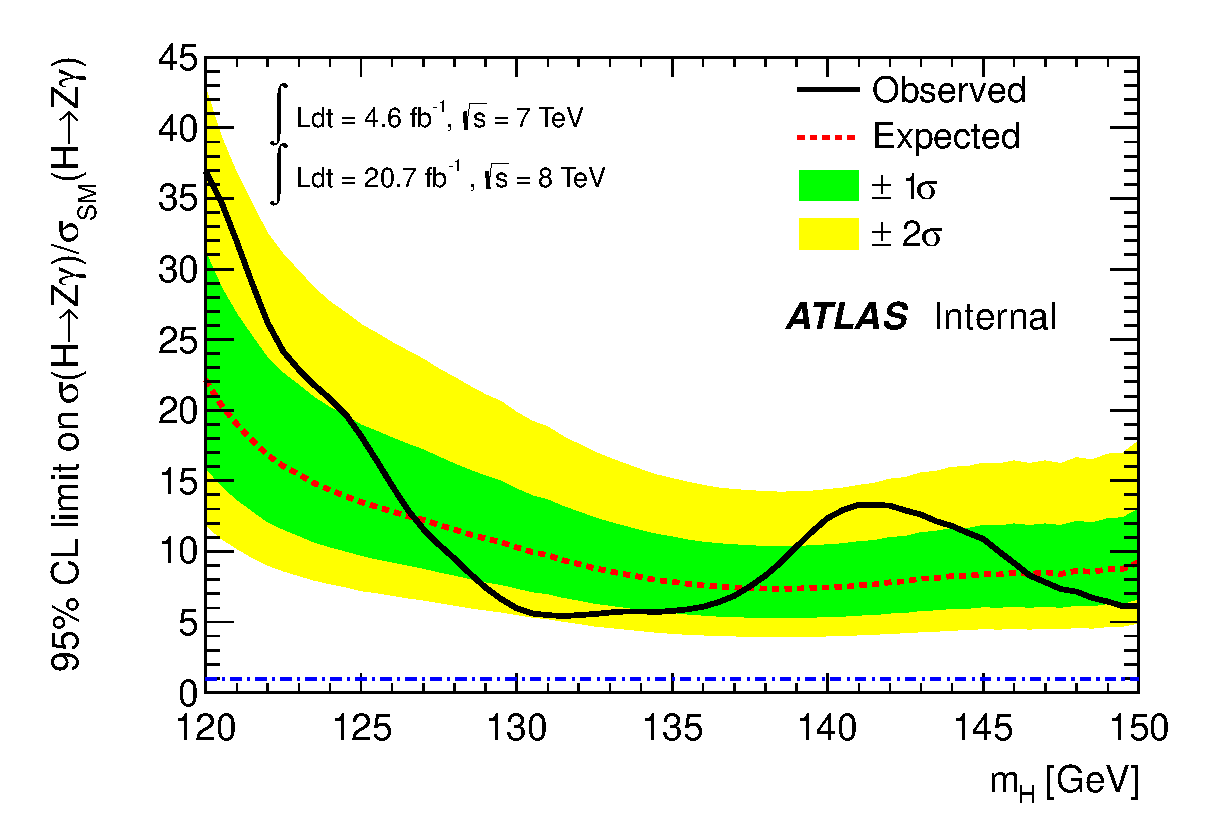
\includegraphics[totalheight=9cm,angle=0]{figures/plot_smooth_cls}
\caption{Observed 95\% $CL$ limits (solid black line) 
  on the production cross section of a SM Higgs boson 
  decaying to $Z\gamma$, as a function of the Higgs boson 
  mass, using \lumiseventev~\ifb\ of $pp$
  collisions at $\sqrt{s}=7$~TeV and \lumieighttev~\ifb\ of $pp$
  collisions at $\sqrt{s}=8$~TeV.
  The median expected 95\% $CL$ exclusion limits (dashed red line)
  are also shown. The green and yellow bands correspond to the $\pm 1\sigma$ 
  and $\pm2\sigma$ intervals.
}
\label{fig:ExpectedExclusion_1}
\end{figure}

\label{sec:results}

\bibliographystyle{atlasnote}
\bibliography{biblio}

\end{document}


